\documentclass[aspectratio=169]{beamer}
%\usetheme{CambridgeUS}
%\usecolortheme{beaver}

%\usefonttheme{serif}
%\usepackage{helvet}

\usefonttheme{serif}     % Font theme: serif
%\usepackage{ccfonts}     % Font family: Concrete Math
\usepackage[T1]{fontenc} % Font encoding: T1

\setbeamersize{text margin left=42pt,text margin right=42pt} 
\setbeamertemplate{navigation symbols}{}
\setbeamertemplate{itemize items}[default]

\beamertemplatenavigationsymbolsempty

\definecolor{fore}{RGB}{51,51,51}
\definecolor{back}{RGB}{255, 254, 250}
\definecolor{title}{RGB}{ 255, 15, 0}
\definecolor{links}{RGB}{18, 168, 255}

\setbeamercolor{titlelike}{fg=title}
\setbeamercolor{normal text}{fg=fore,bg=back}
\setbeamercolor{alerted text}{fg=title}
\setbeamercolor{itemize item}{fg=title}
\setbeamercolor{enumerate item}{fg=title}
\hypersetup{colorlinks,urlcolor=links}

% for code https://kbroman.org/blog/2013/10/07/better-looking-latexbeamer-slides/
\usepackage{listings}
\definecolor{keywords}{RGB}{255,0,90}
\definecolor{comments}{RGB}{60,179,113}
\lstset{language=Python,
keywordstyle=color{keywords},
commentstyle=color{comments}emph}

% fonts
\usepackage[sc]{mathpazo}


% title info
\title{\textbf{Transportation Networks \& Land Use:}}
\subtitle{\textbf{GGR424 - Transportation Geography \& Planning}}
\author{Jeff Allen}
\institute{University of Toronto}
\date{February 7, 2022}


\begin{document}
	
\begin{frame}
	\titlepage	
\end{frame}



\begin{frame}
	
	\textbf{Land Use}
	
	\textbf{Urban Form}
	
	\textbf{Built Environment}
	
	\textbf{Urban Spatial Structure}
	
\end{frame}





\begin{frame}
	
	In transportation geography and planning, we are usually working with \textbf{vector} data (rather than raster data)
	
	\vspace{2mm}
	
	\textbf{Land Use Data}
	
	\begin{itemize}
		\item What is located where
		\item Usually \textbf{Points} or \textbf{Polygons}
	\end{itemize}

	\vspace{2mm}
	
	\textbf{Network Data}
	
	\begin{itemize}
		\item The spatial patterns of transportation networks 
		\item Usually \textbf{Lines} (and nodes/intersections)
	\end{itemize}

	\vspace{2mm}

	\textbf{Travel Data} (more on this next week)
	
	\begin{itemize}
		
		\item Travel Surveys (usually tables, linked to locations)
		\item GPS/Sensor Mobility Data (usually big $N$ point data)

	\end{itemize}
		
\end{frame}





\begin{frame}
	
	\textbf{Land Use Data}
	
	\begin{itemize}
		\item What is located where
		\item Usually \textbf{Points} or \textbf{Polygons}
		\item Many data sources, e.g. OpenStretMap
	\end{itemize}

	\begin{figure}
		\centering
		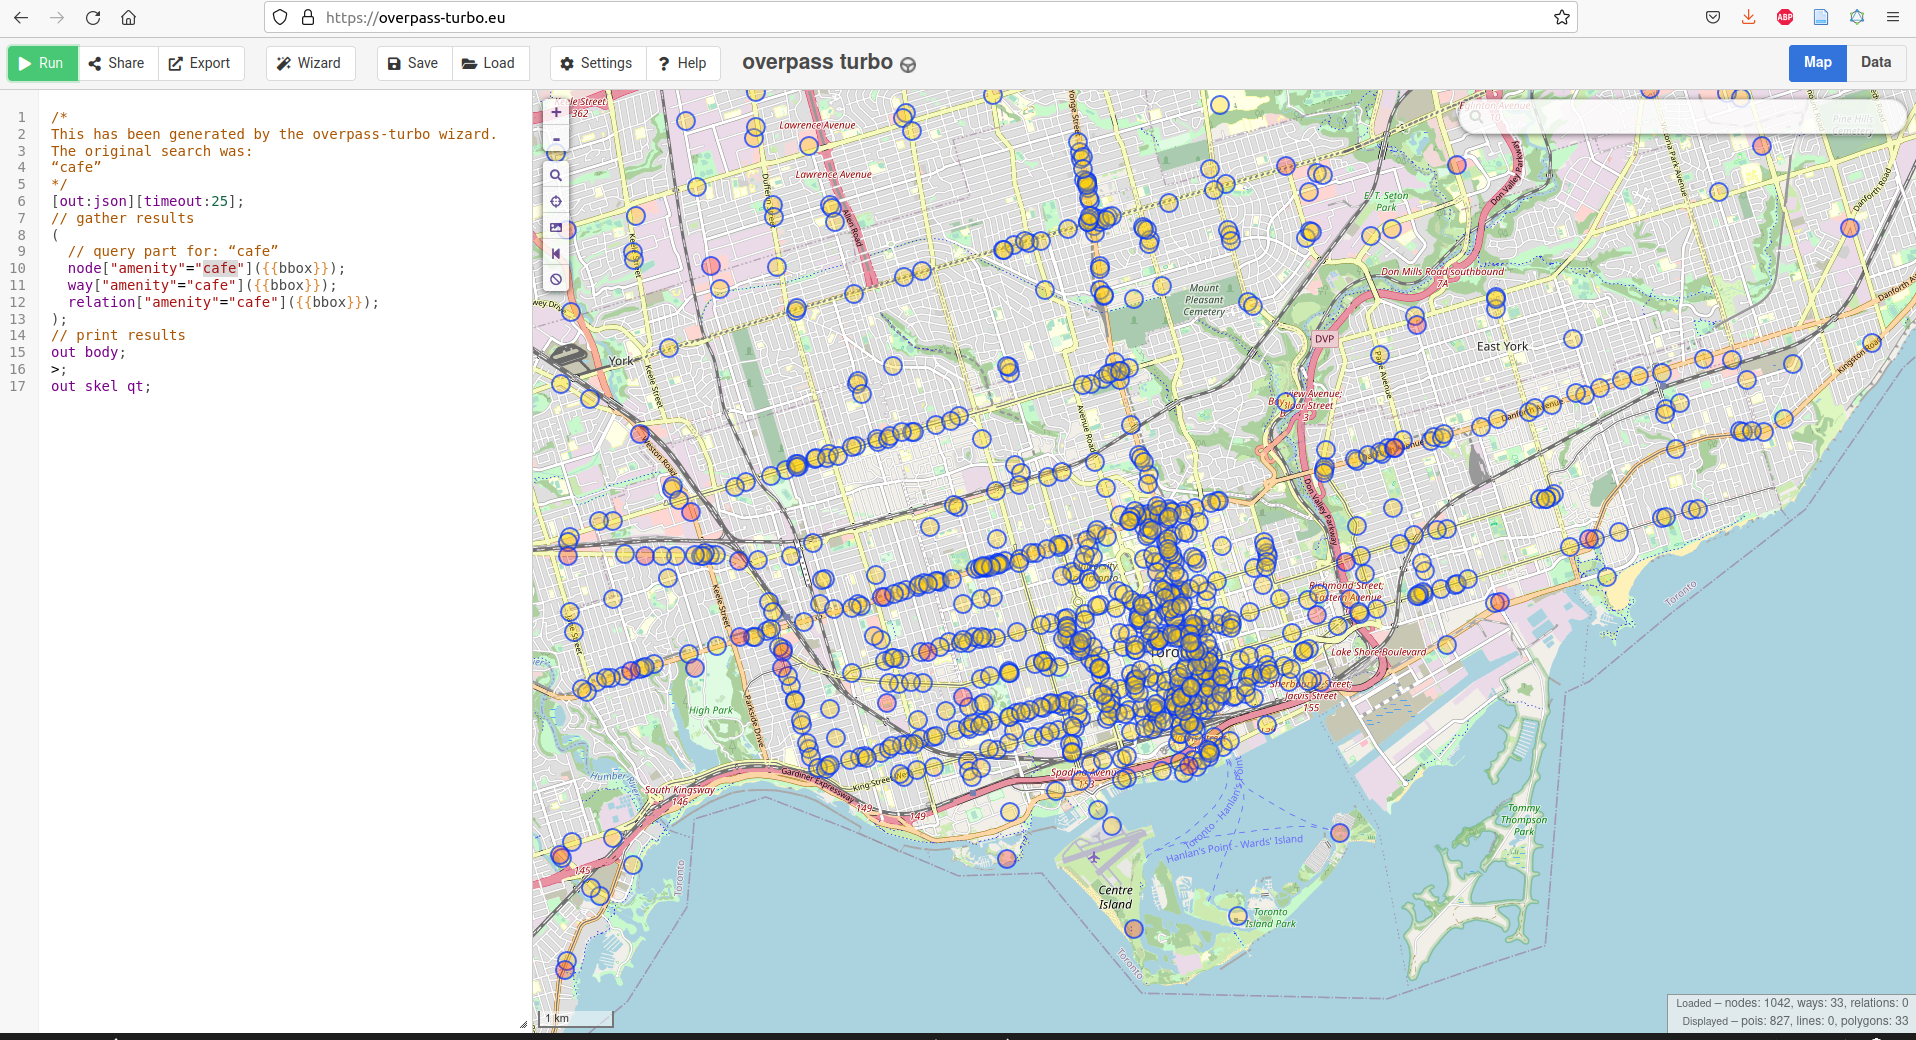
\includegraphics[width=0.9\linewidth]{images/cafe_osm_tor.png}
	\end{figure}
	
	
\end{frame}



\begin{frame}
	
	\textbf{Land Use Data} - e.g. polygon data

	yellow = residential, purple = retail/commercial, blue = industrial, etc. 
	
	\begin{figure}
		\centering
		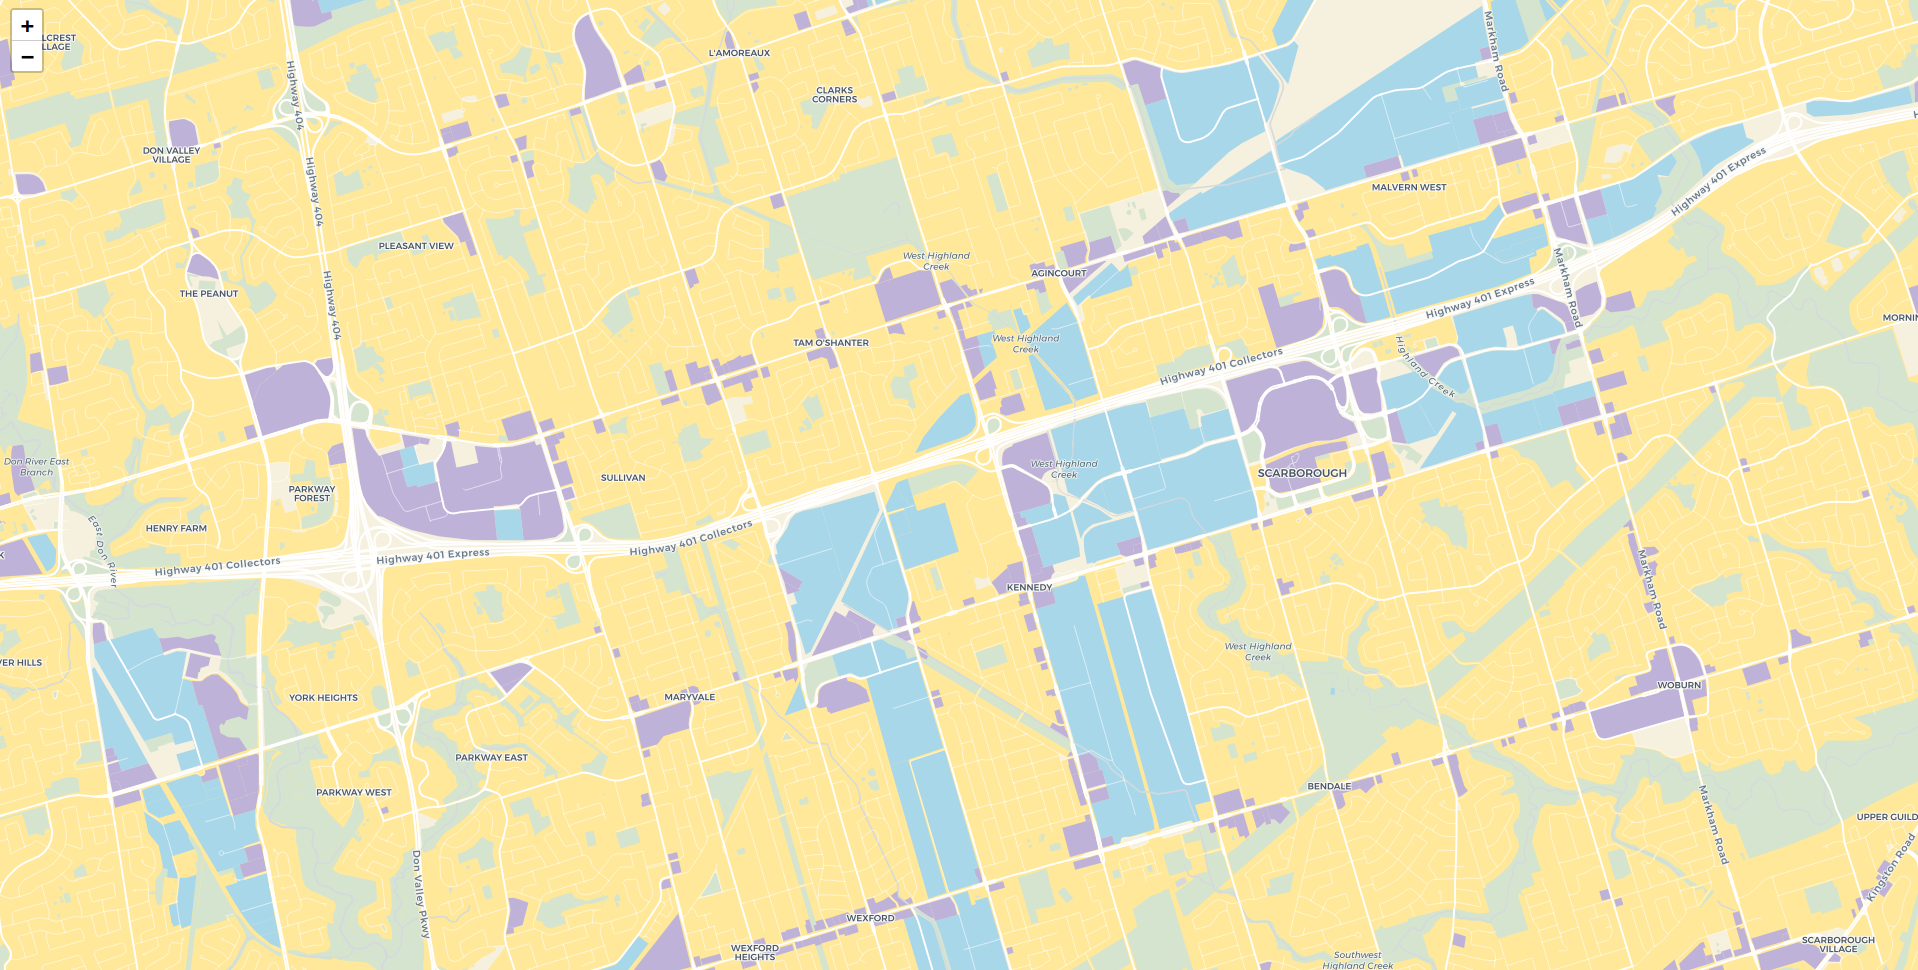
\includegraphics[width=0.9\linewidth]{images/land-use-scarboro.png}
	\end{figure}
	
\end{frame}



\begin{frame}
	
	\textbf{Land Use Data} \\
	
	e.g. polygon data - census data, who lives and works where \\
	
	e.g. point data - libraries in Toronto
	
	\begin{figure}
		\centering
		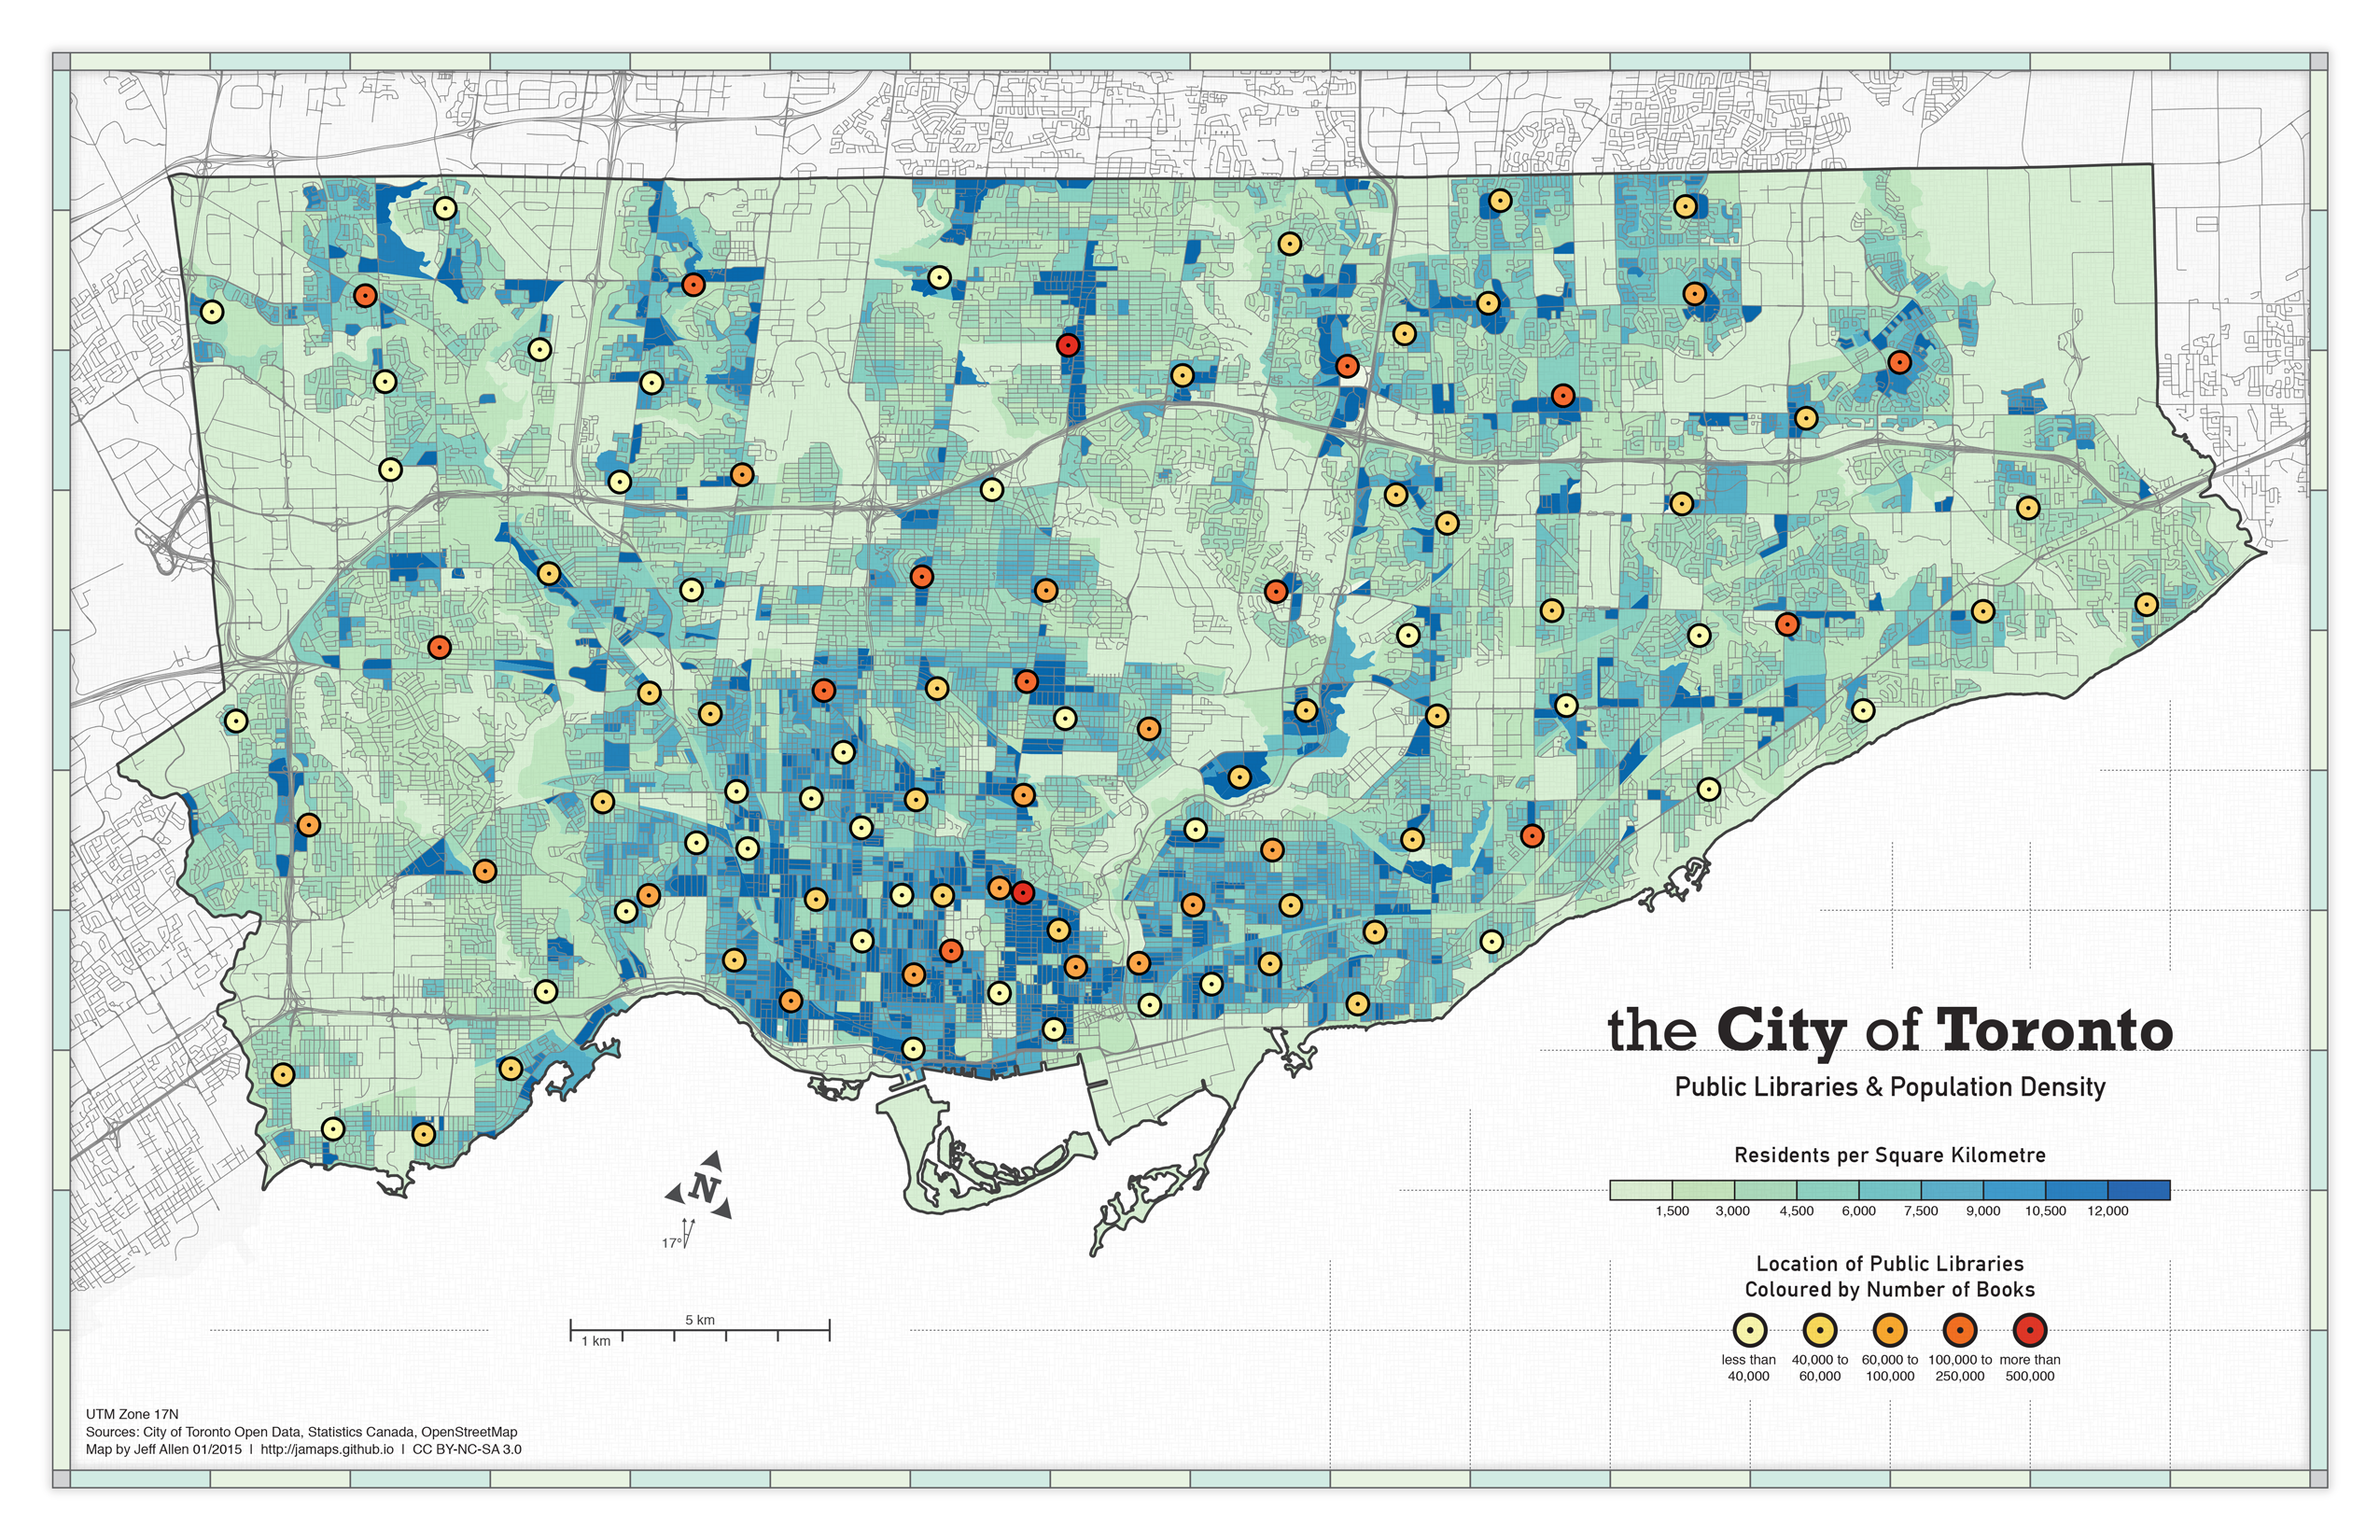
\includegraphics[width=0.8\linewidth]{images/tor_libraries.png}
	\end{figure}
	
	\tiny\url{https://en.wikipedia.org/wiki/Toronto_Public_Library}
	
\end{frame}



% land use data
	
	


\begin{frame}
	
	\begin{columns}
		\begin{column}{0.5\textwidth}
			
			\textbf{Network Data:}
			
			\vspace{6mm}
			
			\textbf{Network} - an interconnected group or system \\
			\vspace{3mm}
			Examples
			\begin{itemize}
				\item Computer network
				\item Social network
				\item Transportation network
				\item Biological network
			\end{itemize} \vspace{3mm}
			Often represented using \textbf{graphs}
		\end{column}
		
		\begin{column}{0.5\textwidth}
			\begin{figure}
				\centering
				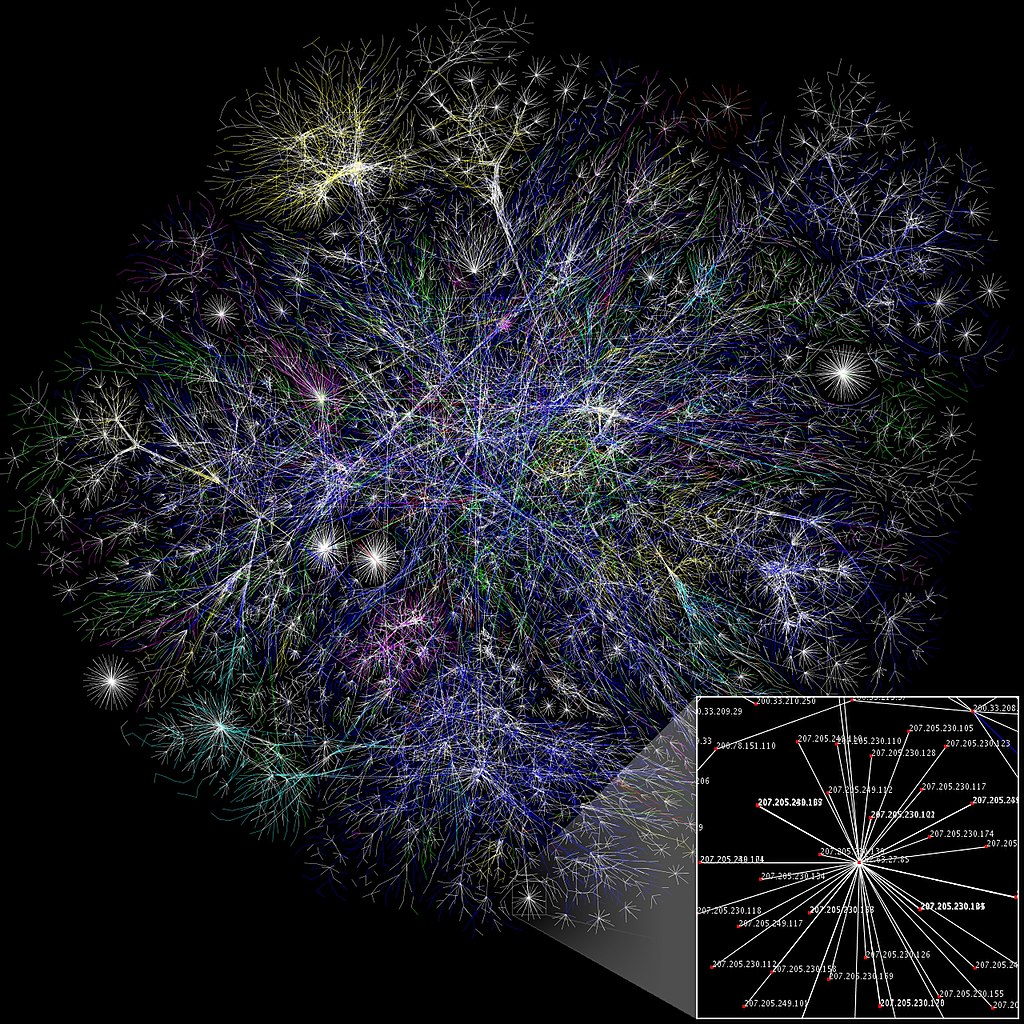
\includegraphics[width=0.9\linewidth]{images/internet}
				\label{fig:internet}
			\end{figure}
			\tiny Source: \url{https://en.wikipedia.org/wiki/Network_science}
		\end{column}
		
	\end{columns}
	
\end{frame}




\begin{frame}
	
	\begin{columns}
		
		\begin{column}{0.5\textwidth}
			
			\textbf{Graph}
			\begin{itemize}
				\item Set of \textit{nodes} (also called points or vertices) and \textit{edges} (also called lines or arcs)
				\item $G = (V, E)$
				\item If two nodes have a relationship, then there is an edge linking them
				\item Edges can have weights (e.g. travel time or speed, surface quality, elevation, etc.)
				\item Graphs can be directed or un-directed (e.g. can have one-way relationship)
			\end{itemize}
			
		\end{column}
		
		\begin{column}{0.4\textwidth}
			\begin{figure}
				\centering
				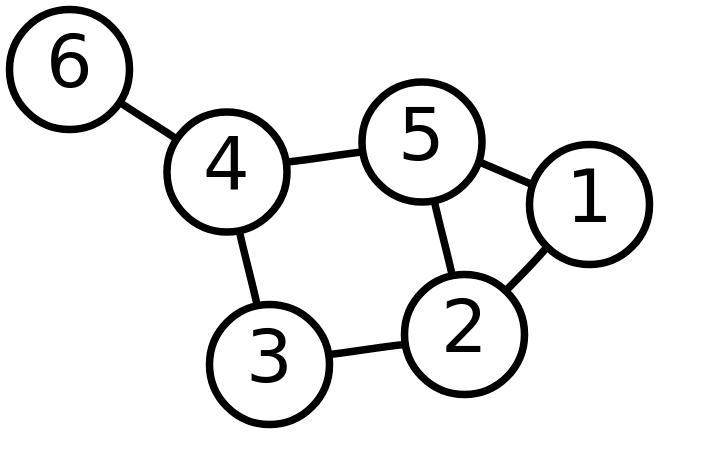
\includegraphics[width=0.9\linewidth]{images/simple_graph}
			\end{figure}
			\tiny Source: \url{https://en.wikipedia.org/wiki/Graph_(discrete_mathematics)}
		\end{column}	
		
	\end{columns}
	
\end{frame}





\begin{frame}
	
	\small Can you walk across all of the seven bridges in K\"onigsberg, without ever repeating a single bridge in the course of one's walk? (Leonhard Euler, 1736)
	
	\begin{figure}
		\centering
		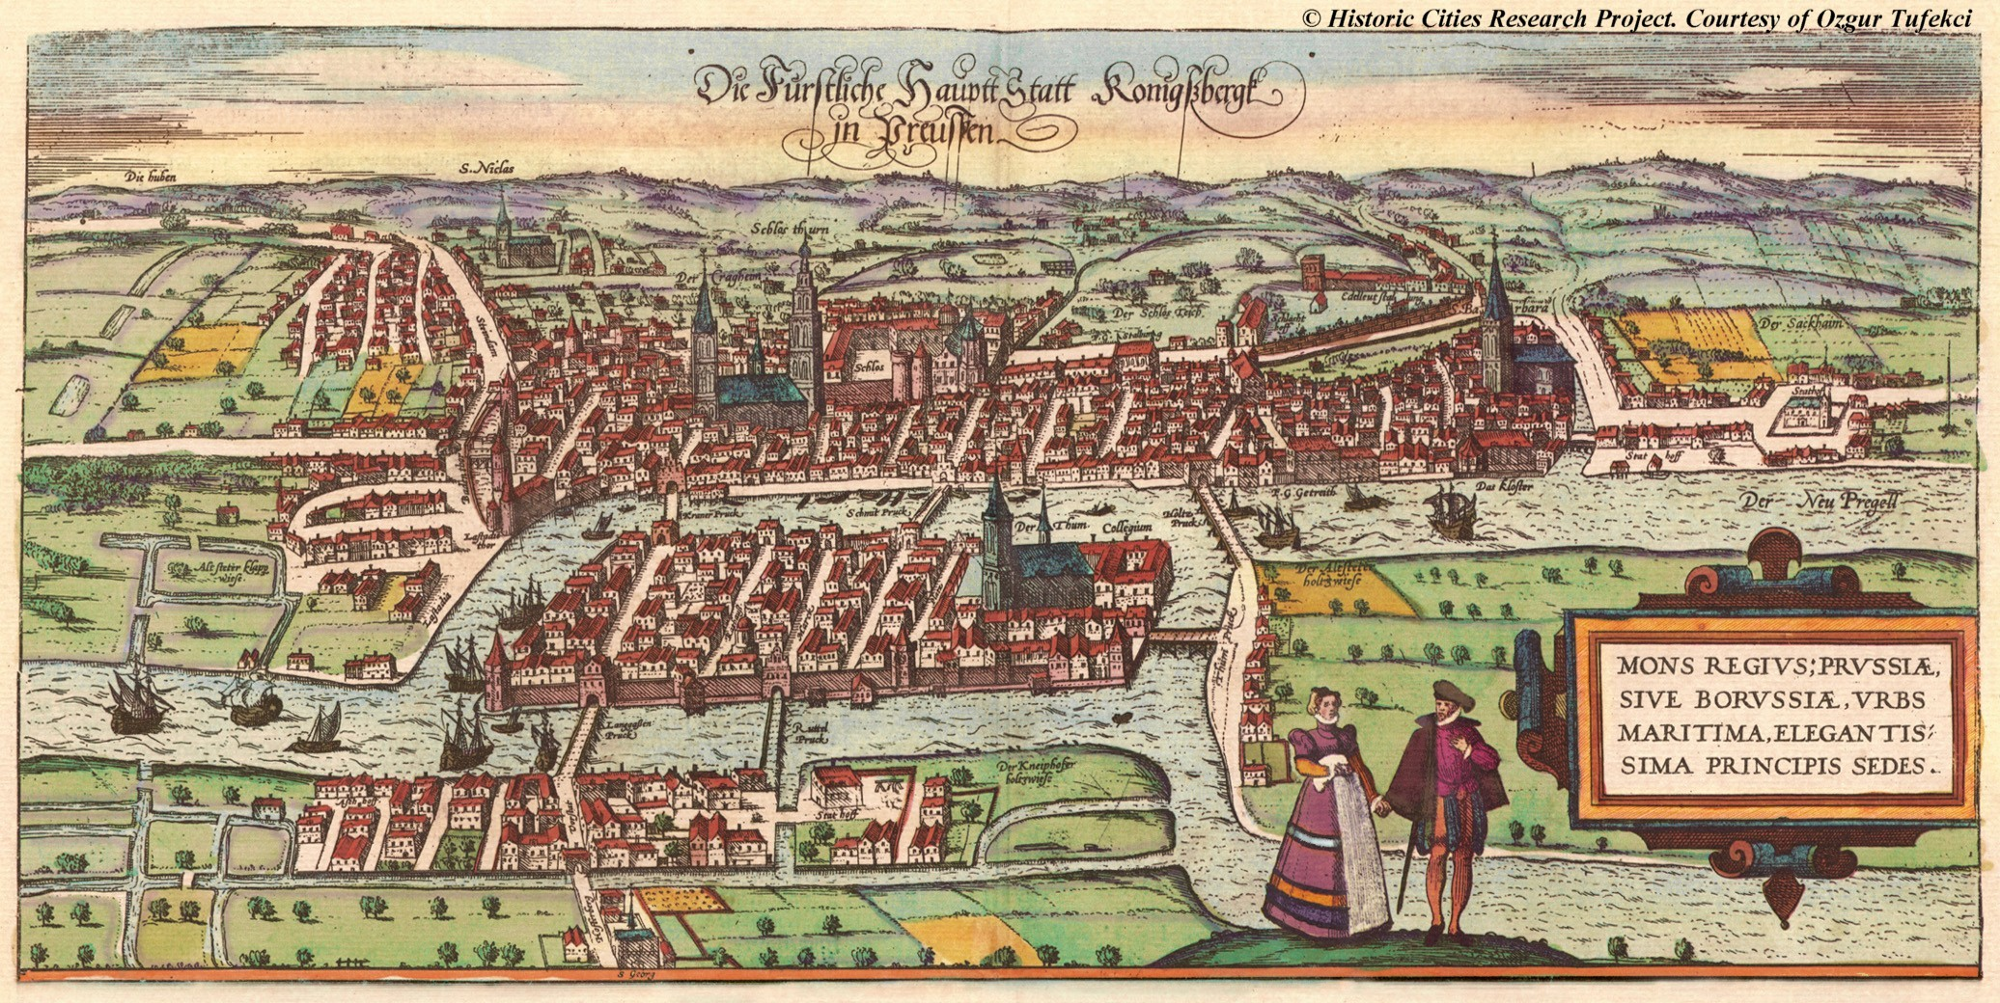
\includegraphics[width=0.9\linewidth]{images/konigsberg_1}
	\end{figure}
	\tiny \tiny Source: \url{https://medium.com/basecs/konigsberg-seven-small-bridges-one-giant-graph-problem-2275d1670a12}
	
\end{frame}




 


\begin{frame}
	
	\small Can you walk across all of the seven bridges in K\"onigsberg, without ever repeating a single bridge in the course of one's walk? (Leonhard Euler, 1736)
	
	\vspace{2mm}
	
	\small Representing K\"onigsberg as a graph
	
	\begin{columns}
		
		\begin{column}{0.5\textwidth}
			
			\begin{figure}
				\centering
				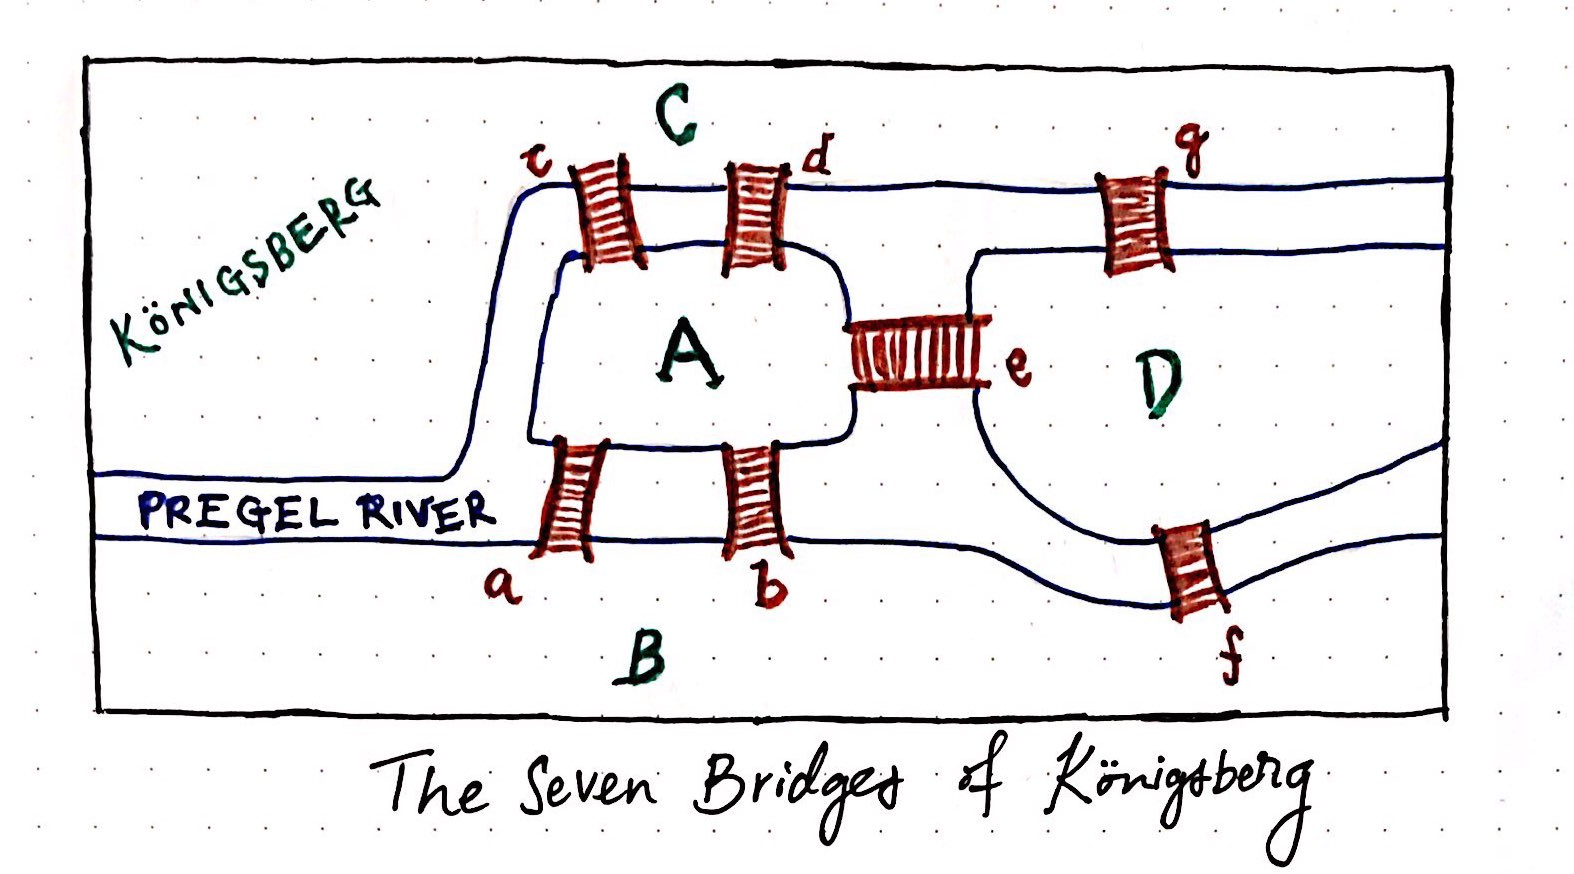
\includegraphics[width=1.1\linewidth]{images/konigsberg_2}
			\end{figure}
			
		\end{column}
		
		\begin{column}{0.5\textwidth}
			\begin{figure}
				\centering
				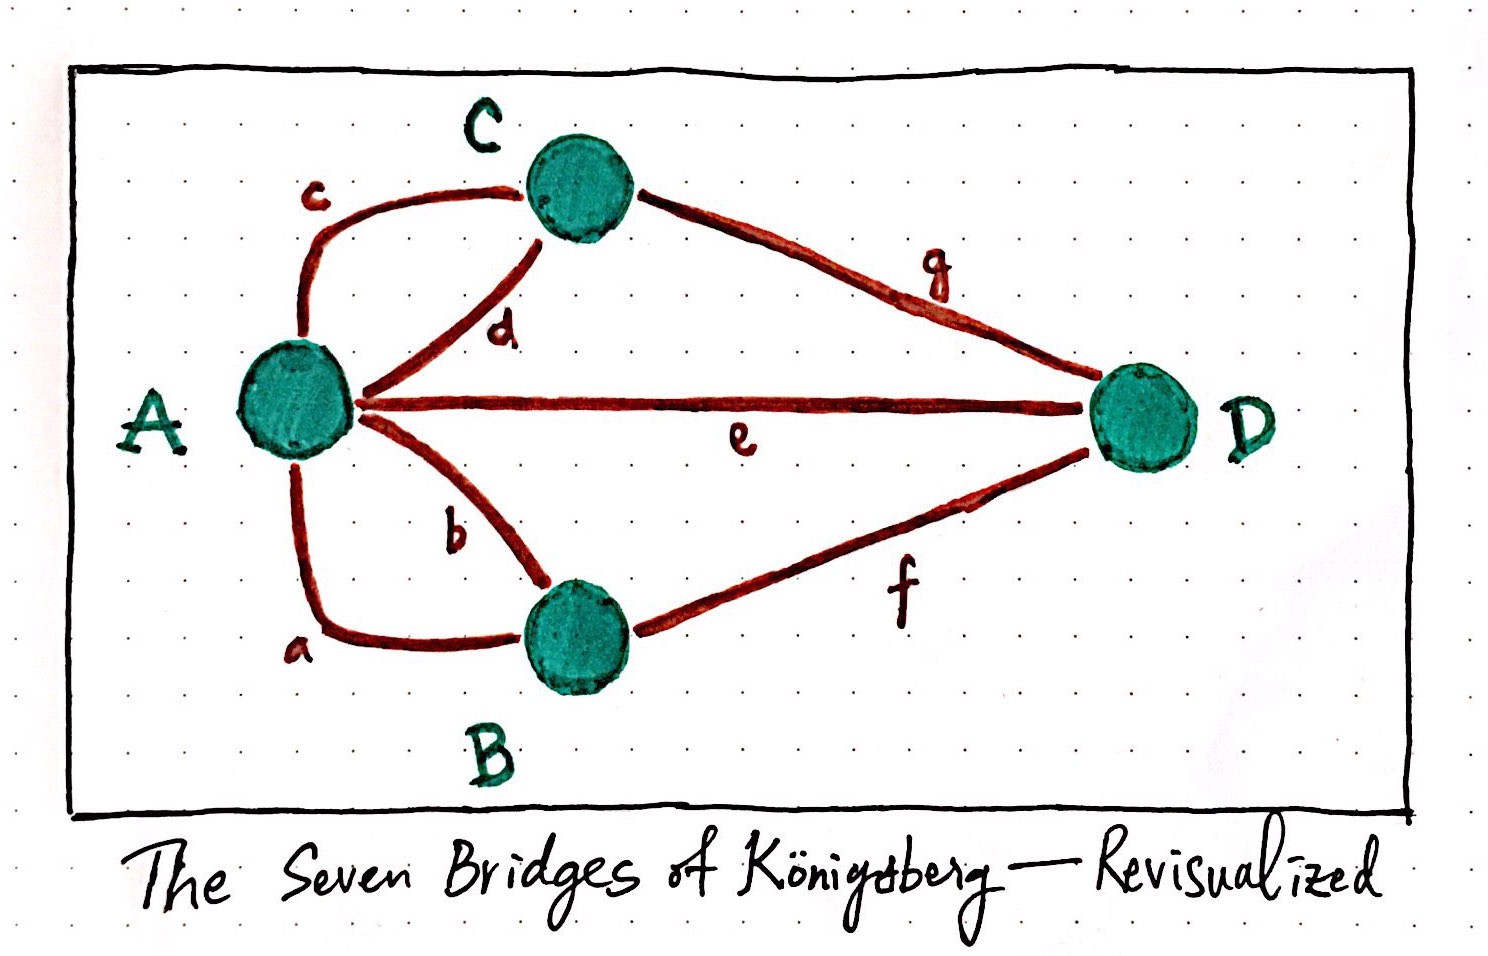
\includegraphics[width=1.0\linewidth]{images/konigsberg_3}
			\end{figure}
		\end{column}
		
	\end{columns}
	\vspace{4mm}
	\tiny \tiny Source: \url{https://medium.com/basecs/konigsberg-seven-small-bridges-one-giant-graph-problem-2275d1670a12}
\end{frame}




\begin{frame}
	
	\begin{figure}
		\centering
		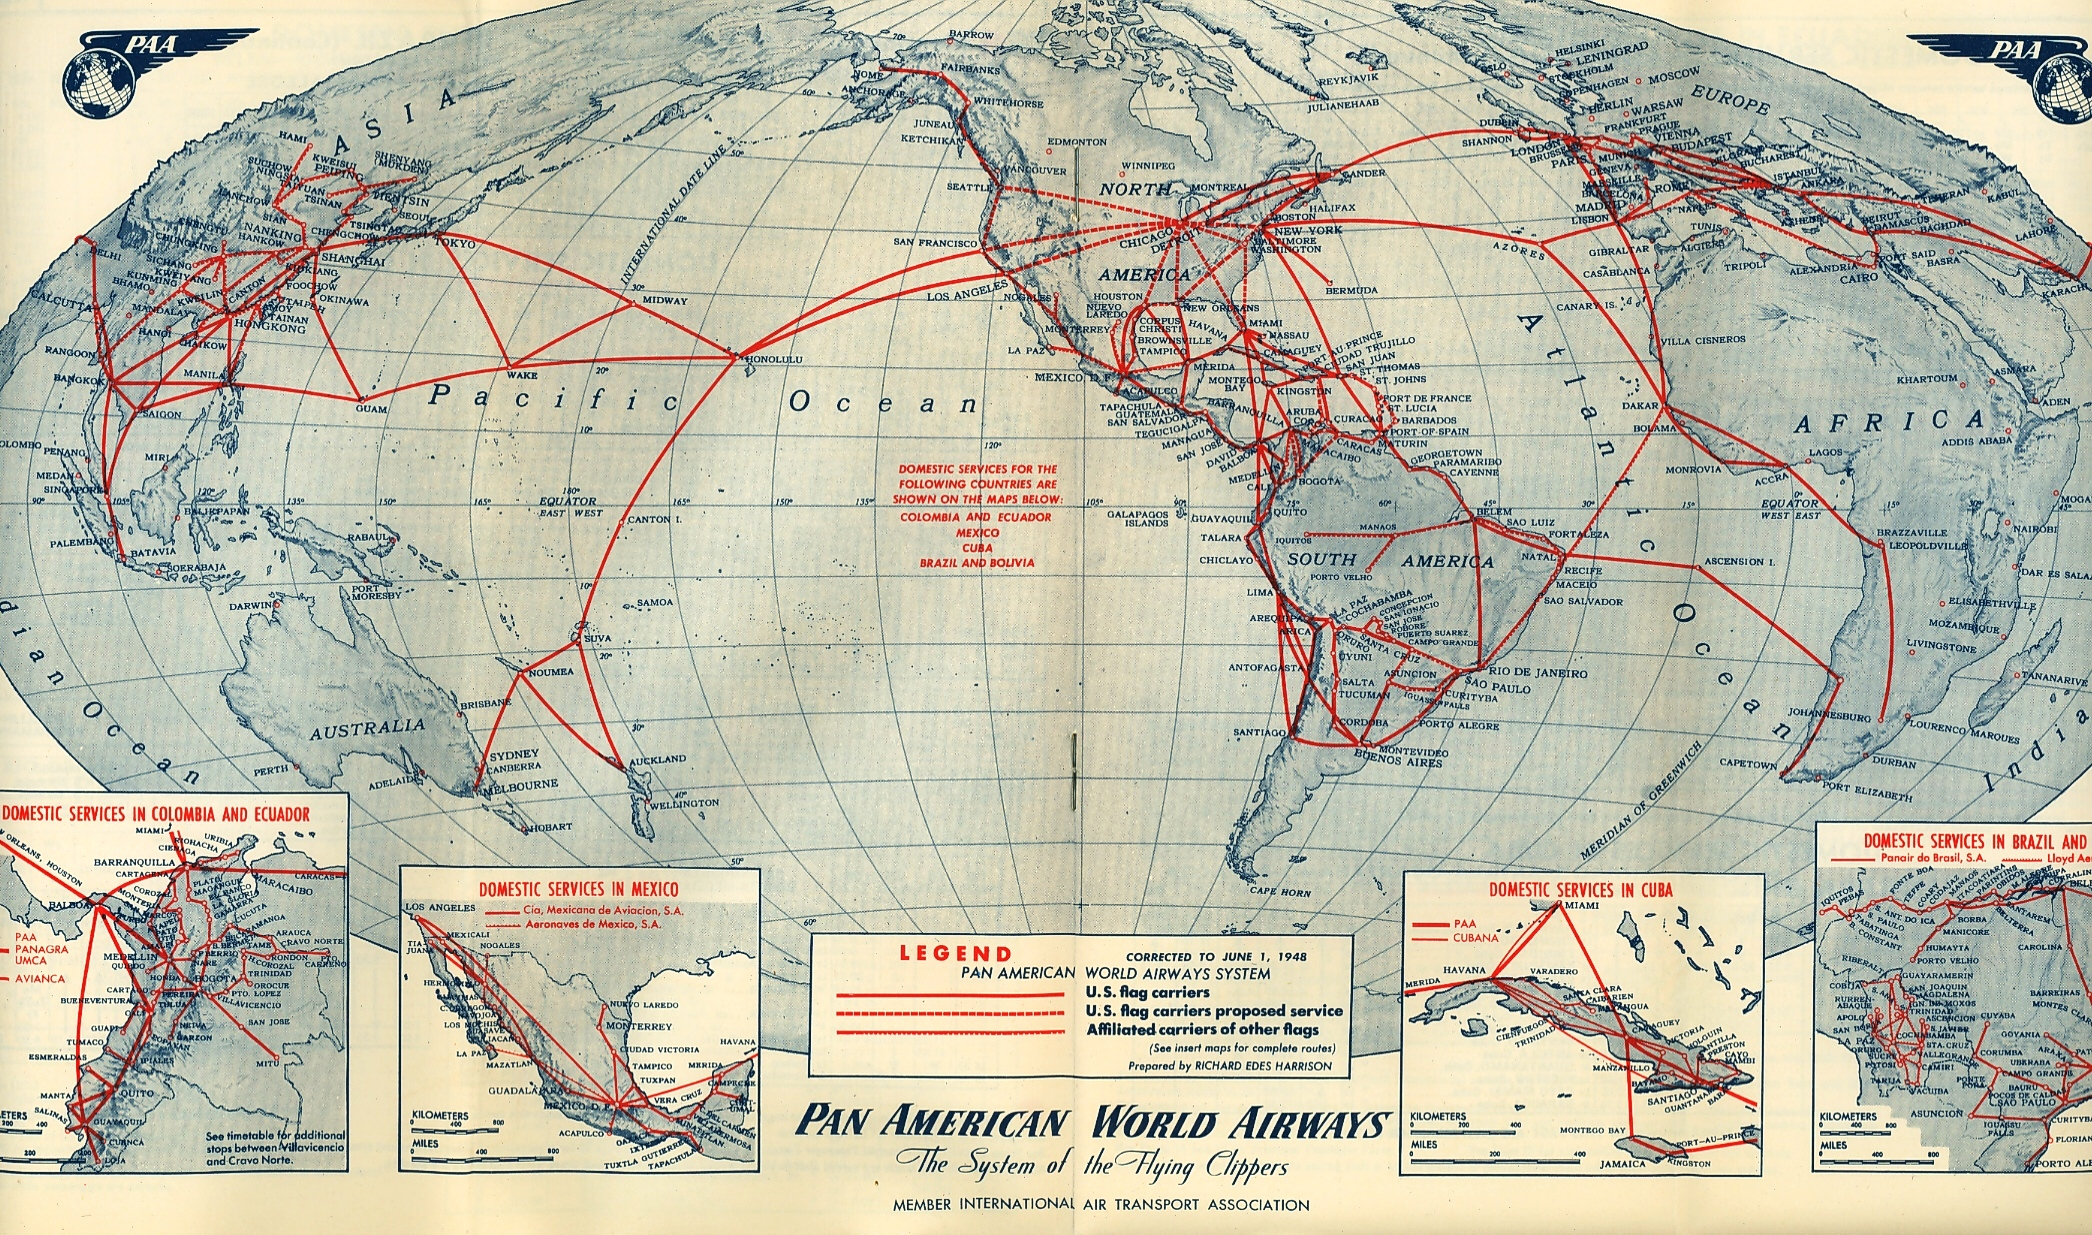
\includegraphics[width=1\linewidth]{images/flight_path_panam_1948}
	\end{figure}
	
\end{frame}




\begin{frame}

	
	\begin{columns}
		\begin{column}{0.5\textwidth}
			In transportation geography and planning, network data are used for measuring distances and travel times over \textit{network} space.
			\vspace{2mm}
			
			These distances/times can be used for a range of analyses
			
			\vspace{4mm}
			
			\tiny Source: \url{https://www.openstreetmap.org}
		\end{column}
		\begin{column}{0.5\textwidth}
			
			\begin{figure}
				\centering
				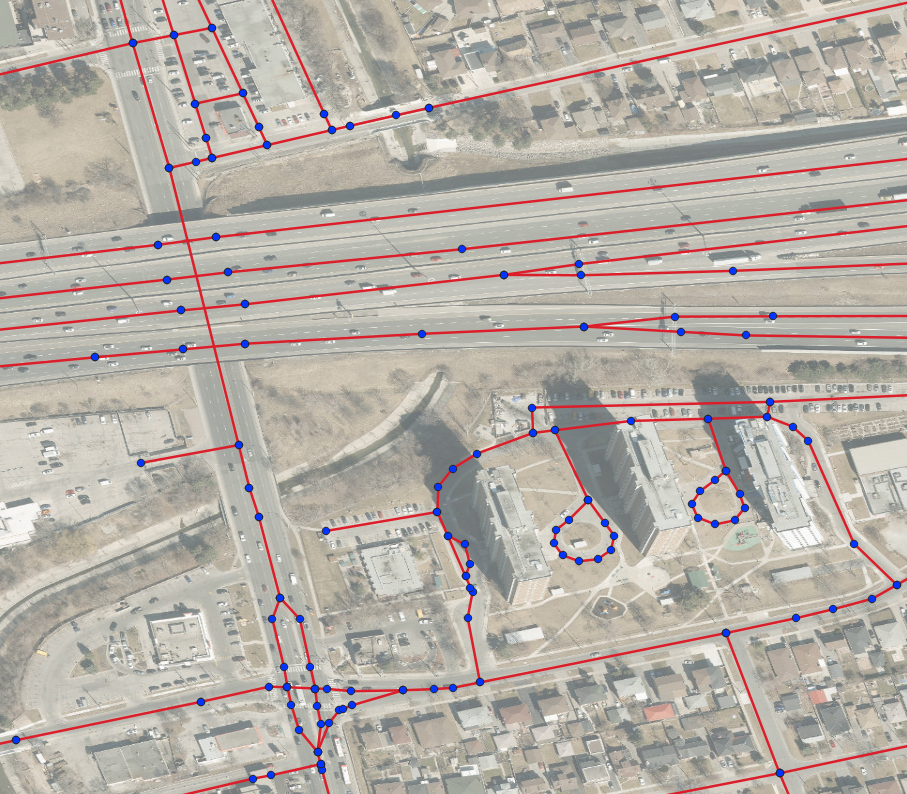
\includegraphics[width=1\linewidth]{images/network_tor_eg}
			\end{figure}
			
		\end{column}
	\end{columns}
	
	
\end{frame}




\begin{frame}
	
	\textbf{Transportation network data sources:}
	
	\vspace{2mm}
	
	Driving
	\begin{itemize}
		\item OpenStreetMap (free and detailed, depending on crowdsourced activity)
		\item Government sources (e.g. City of Toronto Centreline, Federal Road Network Files)
		\item Proprietary Networks (e.g. HERE, DMTI, Google Maps, etc.). Often used if needing travel times with congestion
	\end{itemize}

	Walking \& Cycling
	\begin{itemize}
		\item OpenStreetMap (free and detailed, depending on crowdsourced activity)
		\item Various municipal gov't data sources
	\end{itemize}

	Transit 
	\begin{itemize}
		\item GTFS (General Transit Feed Specification)
	\end{itemize}
	
\end{frame}





\begin{frame}
	
	
	\begin{columns}
		\begin{column}{0.5\textwidth}
			\textbf{Network Distance}
			
			\begin{itemize}
				\item The distance or travel time between two points, based on the \textit{shortest-path} in a network graph.
				\item Included in many mapping applications and software (e.g. Google Maps, Uber, etc.)
				\item Different than straight-line (e.g. Euclidean) distance
			\end{itemize}
			\vspace{4mm}
			\tiny Source: \url{https://www.openstreetmap.org}
		\end{column}
		\begin{column}{0.5\textwidth}
			
			\small \textit{shortest-path} by walking (22 min, 1.8 km)
			\begin{figure}
				\centering
				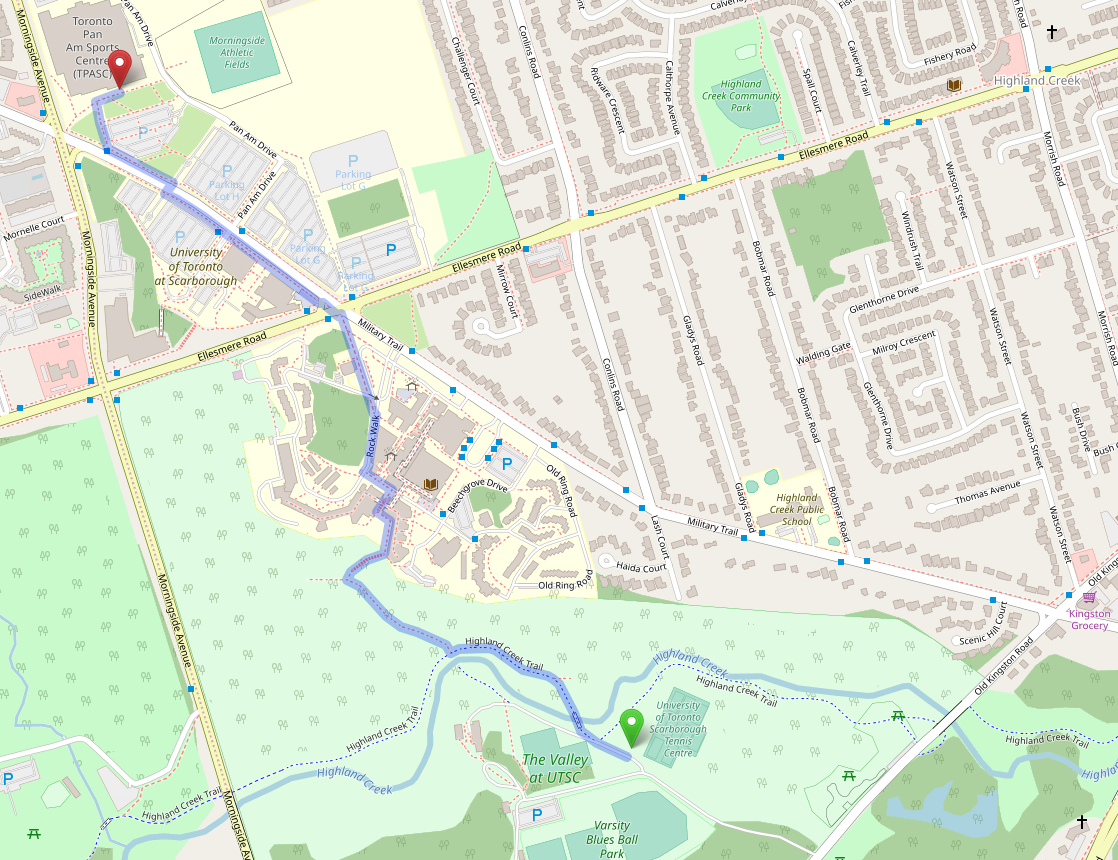
\includegraphics[width=1\linewidth]{images/route_utsc_walk}
			\end{figure}
		\end{column}
	\end{columns}

\end{frame}





\begin{frame}
	
	\begin{columns}
		\begin{column}{0.5\textwidth}
			\small \textit{shortest-path} by bicycle (12 min, 2.5 km)
			\begin{figure}
				\centering
				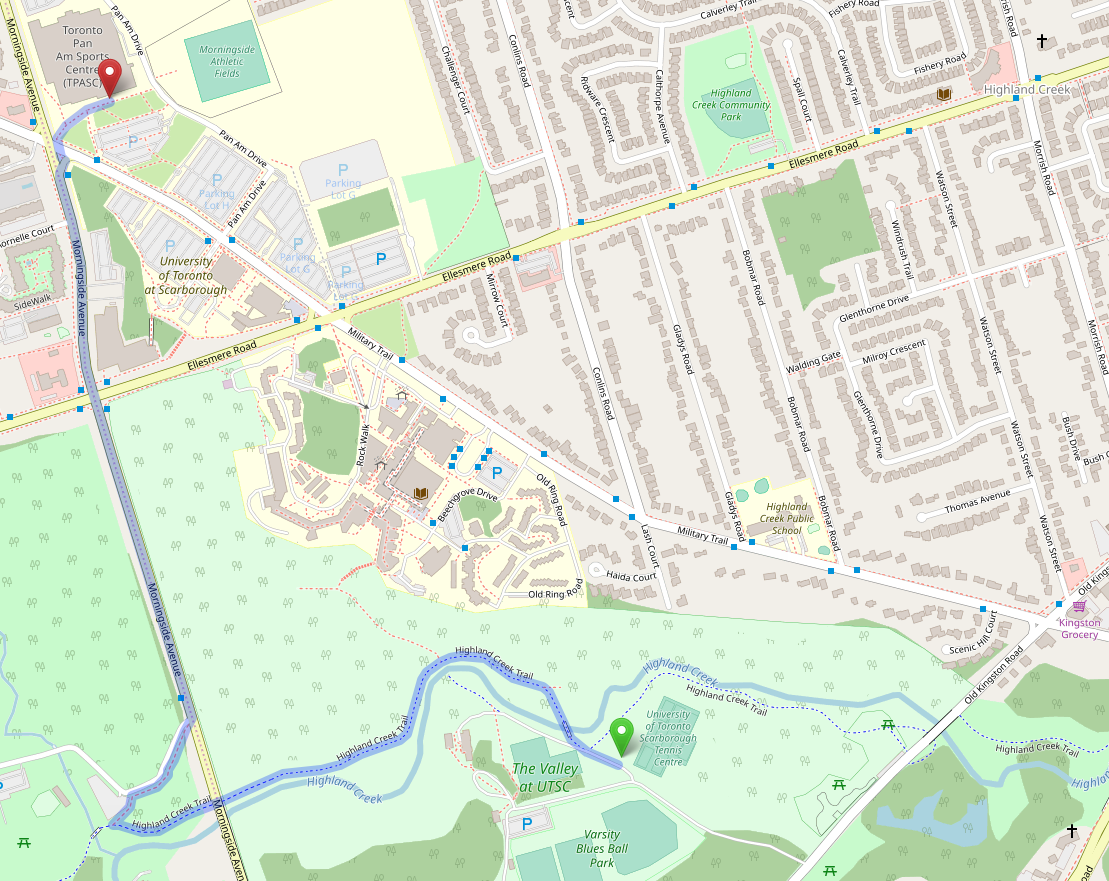
\includegraphics[width=1\linewidth]{images/route_utsc_bike}
			\end{figure}
		\end{column}
		\begin{column}{0.5\textwidth}
			
			\small \textit{shortest-path} by car (8 min, 3.0 km)
			\begin{figure}
				\centering
				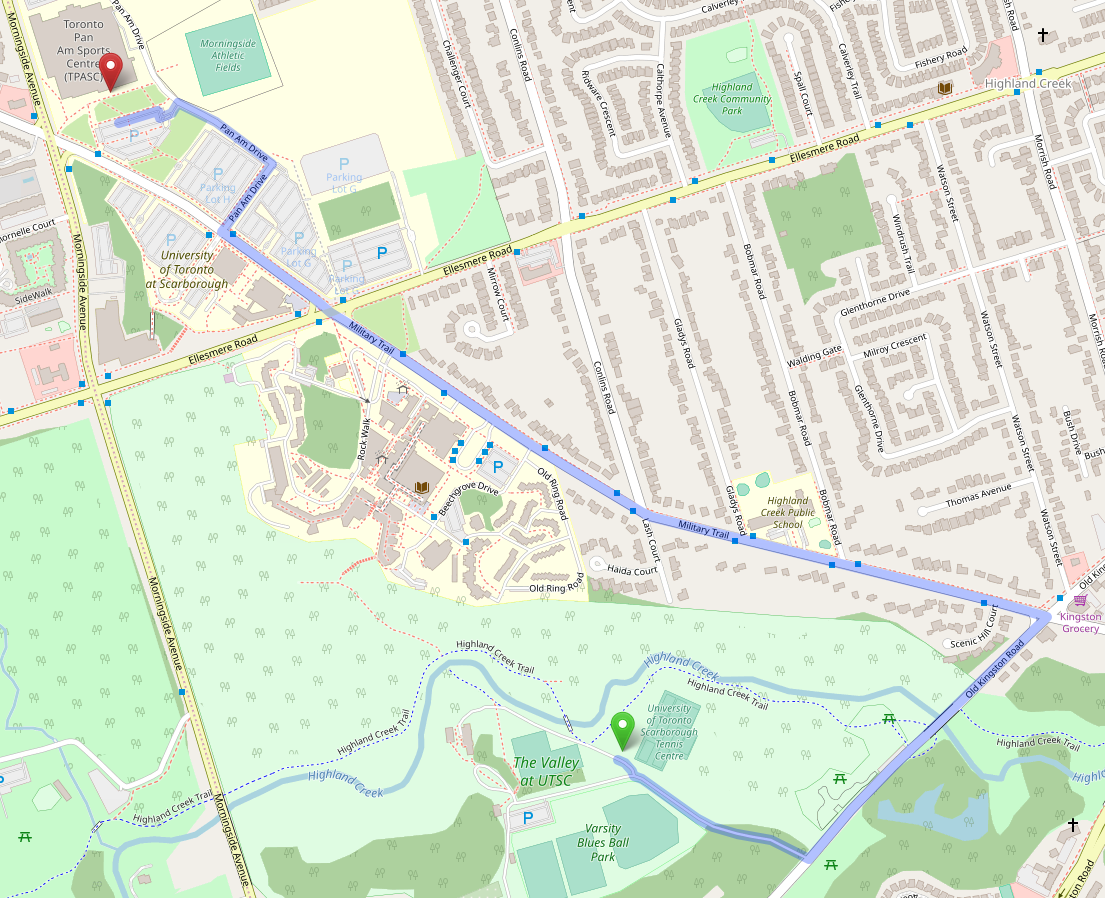
\includegraphics[width=1\linewidth]{images/route_utsc_car}
			\end{figure}
		\end{column}
	\end{columns}


\end{frame}




\begin{frame}
	
	\textbf{Shortest Path Analysis}
	
	\begin{itemize}
		\item Finding the "shortest" path between A and B
		\item "shortest" can be in distance, time, other costs, or combination of costs
		\item Several different algorithms (e.g. Dijkstra)
		
	\end{itemize}
	
	\begin{figure}
		\centering
		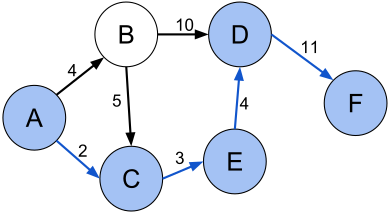
\includegraphics[width=0.5\linewidth]{images/shortest_path}
	\end{figure}

	\tiny\url{https://en.wikipedia.org/wiki/Dijkstras_algorithm}
	
	\tiny\url{https://en.wikipedia.org/wiki/Shortest_path_problem}	

\end{frame}




\begin{frame}

	\begin{figure}
		\centering
		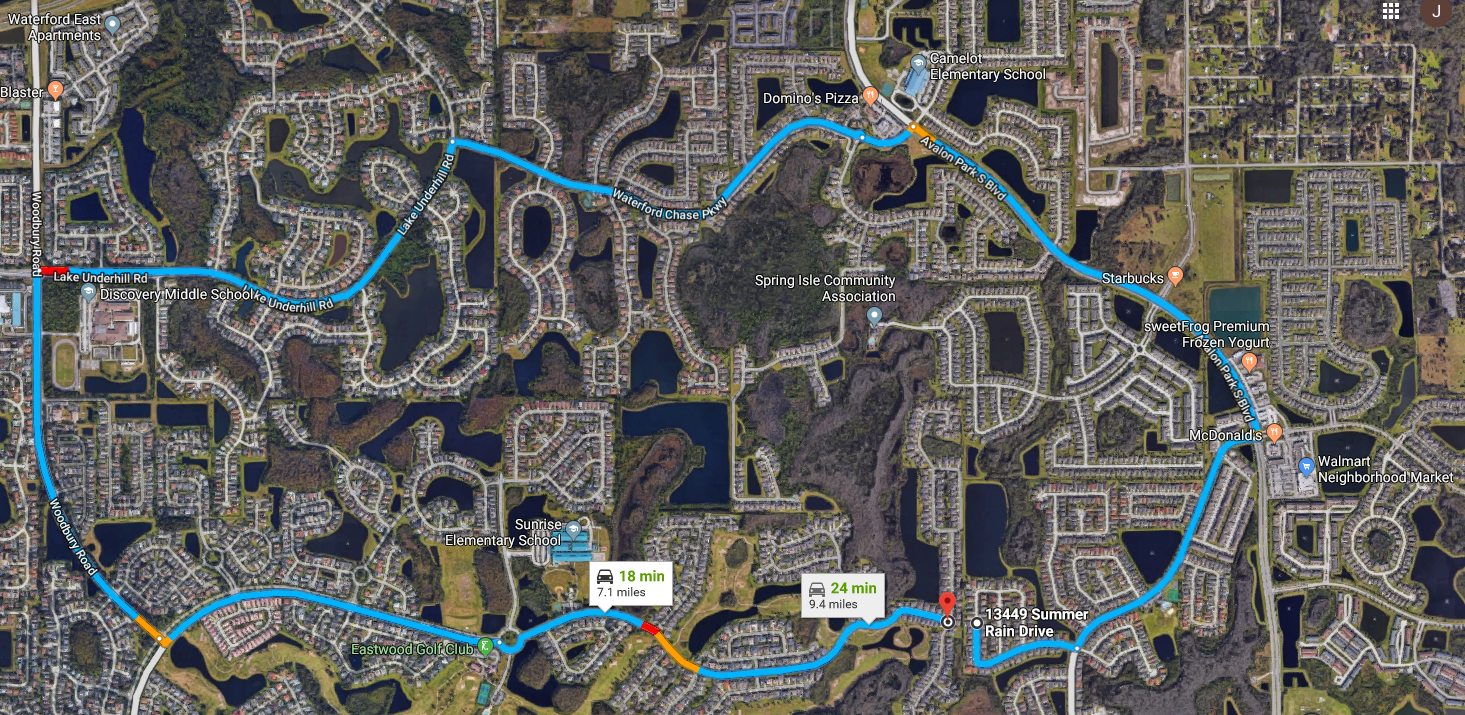
\includegraphics[width=0.95 \linewidth]{images/orlando}
	\end{figure}
	\tiny \url{https://www.google.ca/maps/dir/28.5327099,-81.1608841/28.5326847,-81.1618508/@28.5363151,-81.1840563,6816m/data=!3m1!1e3!4m3!4m2!3e0!5i1}
\end{frame}


\begin{frame}
	
	\begin{figure}
		\centering
		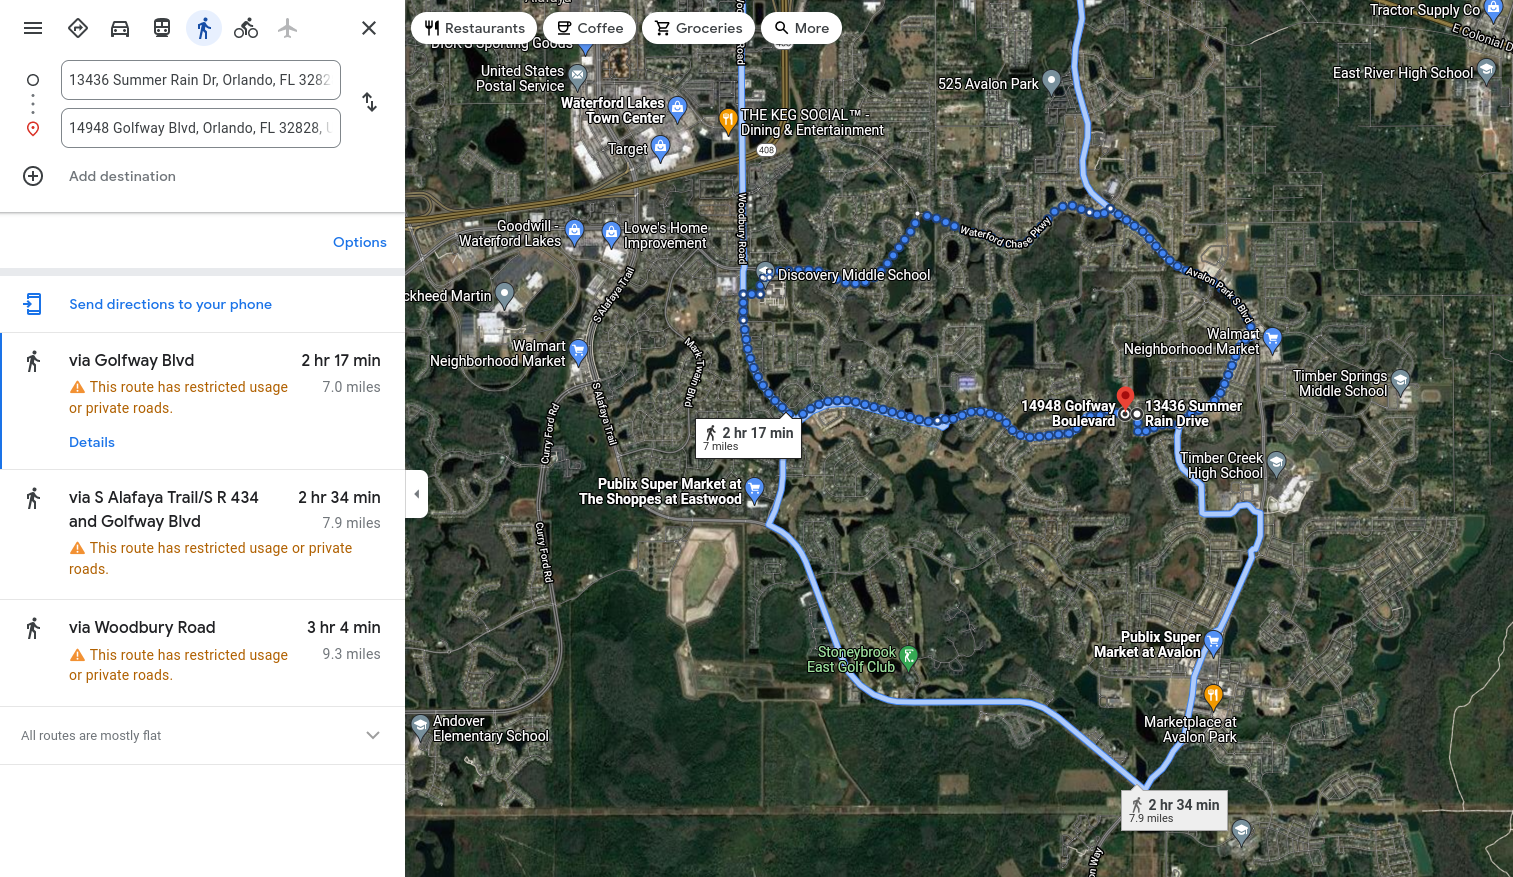
\includegraphics[width=0.95 \linewidth]{images/stupid_route_orlando}
	\end{figure}
	\tiny \url{https://www.google.ca/maps/dir/28.5327099,-81.1608841/28.5326847,-81.1618508/@28.5363151,-81.1840563,6816m/data=!3m1!1e3!4m3!4m2!3e0!5i1}
\end{frame}








\begin{frame}

	\textbf{Closest Facility Analysis} - finding the nearest location(s) from a set of locations distributed over space \\
	\vspace{3mm}
	Often used in medical and emergency services. 
	\begin{itemize}
		\item e.g. which fire station is closest to a fire
		\item e.g. what is the nearest emergency room
	\end{itemize}
\end{frame}



\begin{frame}
	
	e.g. in Ottawa, is UofO or Carleton closer to where you live?
	
	\begin{figure}
		\centering
		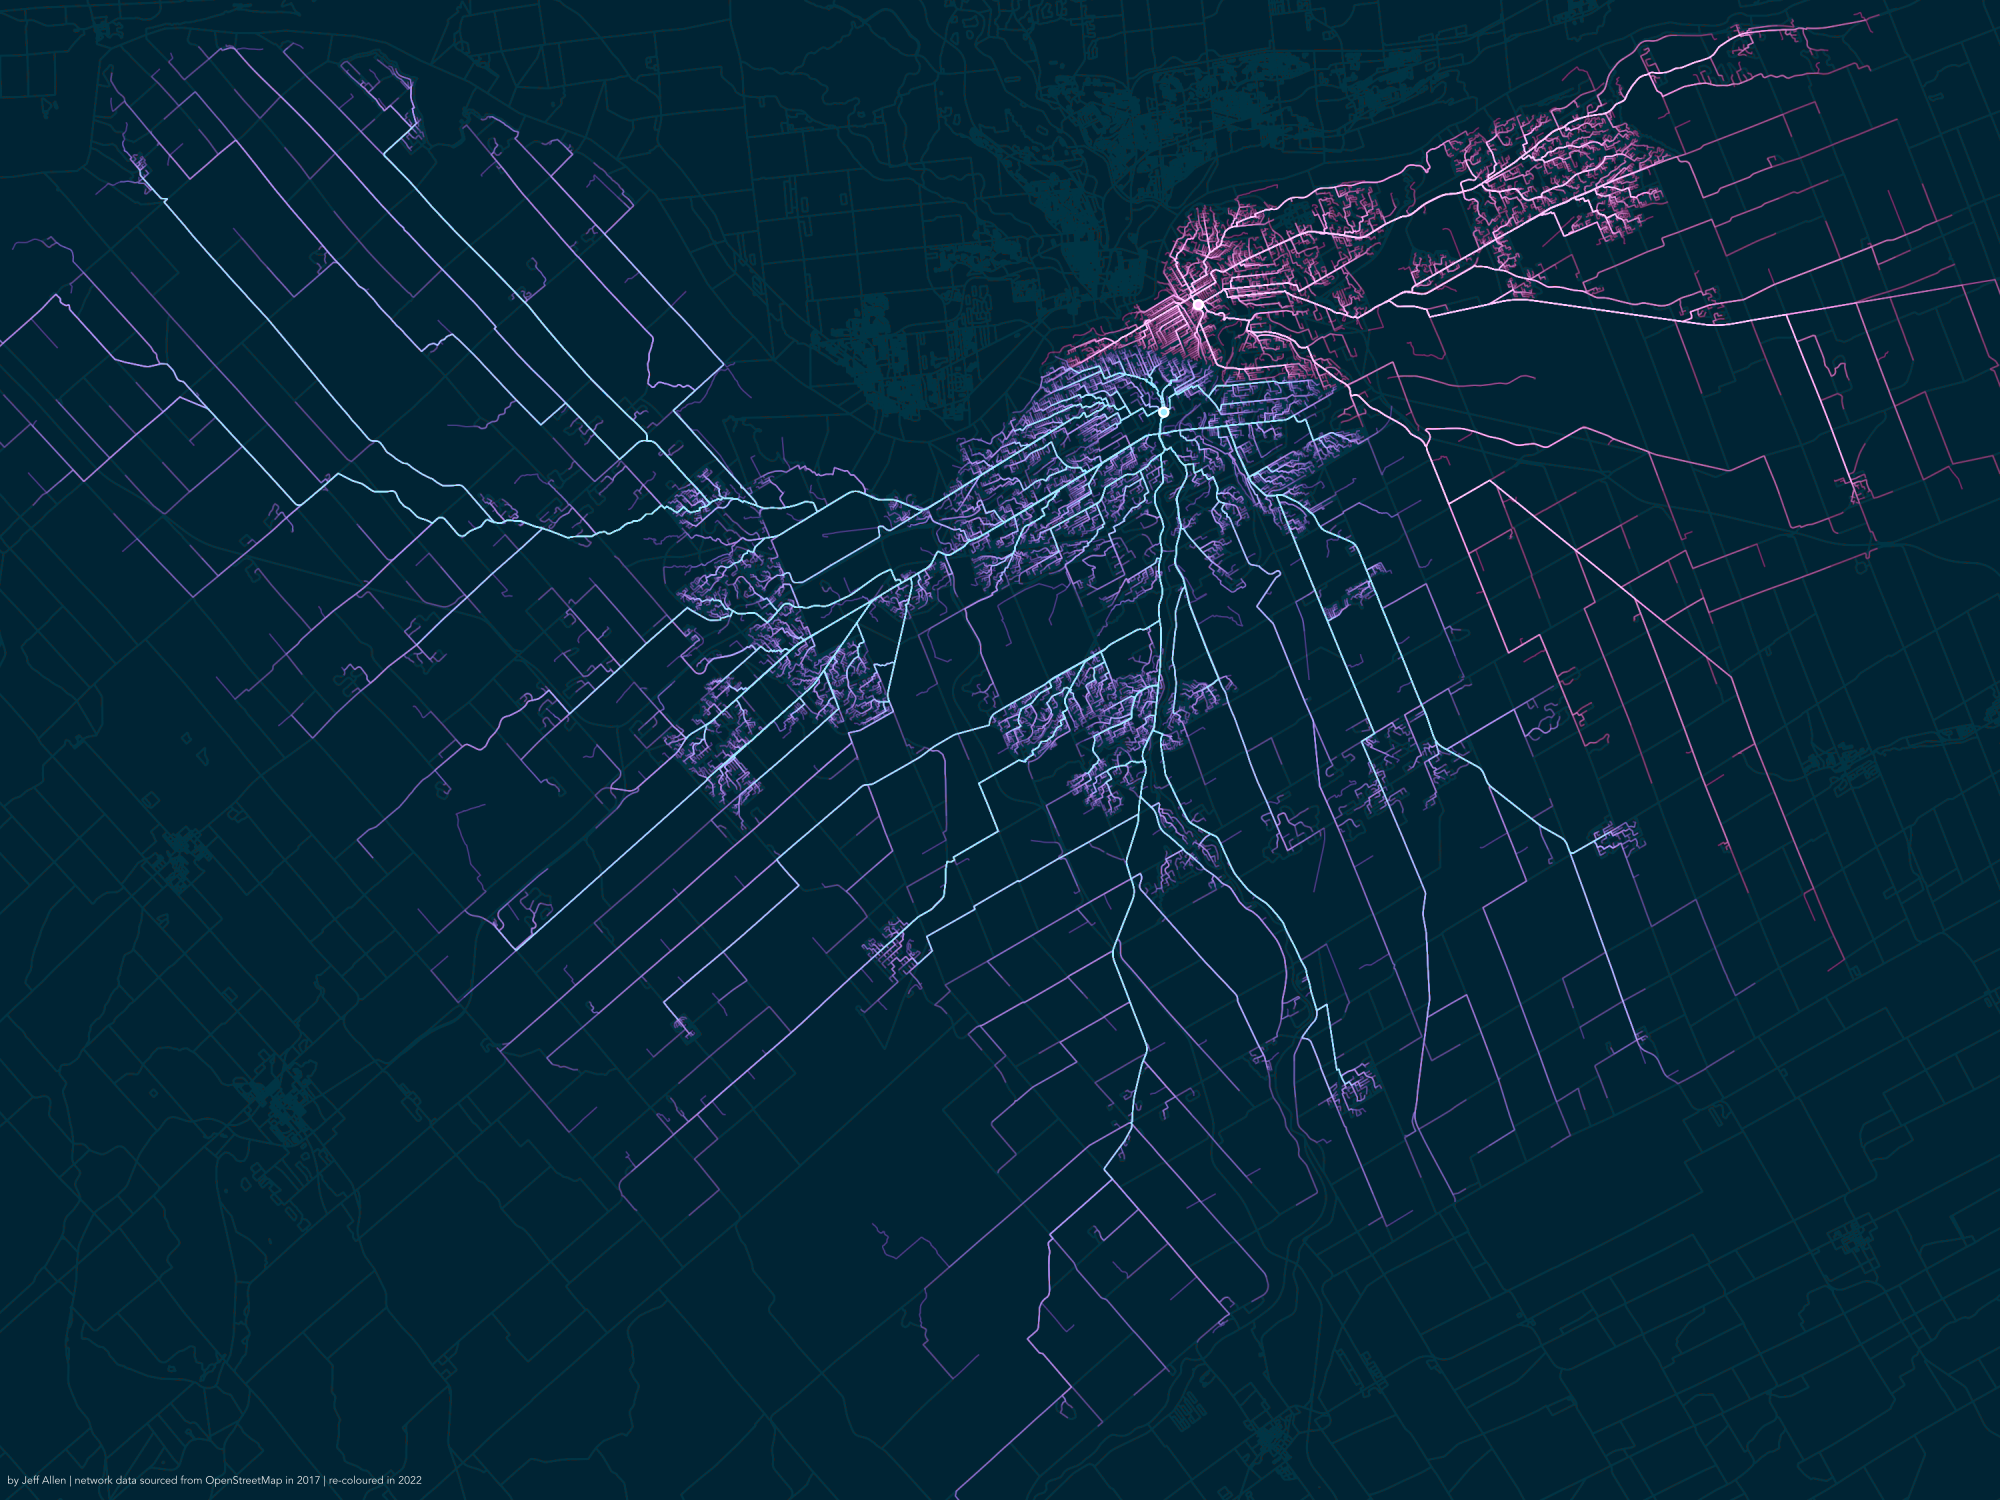
\includegraphics[width=0.79\linewidth]{images/ottawa_2c.png}
	\end{figure}
	\tiny \url{}
\end{frame}





\begin{frame}

	
	\textbf{Location Allocation}
	\begin{itemize}
		\item Procedures for determining the optimal location for one or more facilities that will service demand from a given set of points across space
		\item Often used in planning new locations of retail, public facilities, distribution centres, etc.
		\item Often use network distances + other data (e.g distributions of population)
	\end{itemize}
	
\end{frame}





\begin{frame}

	
	\textbf{Travelling Salesman}
	
	\begin{itemize}
		\item 	Given a list of locations, and the (network) distances between each pair of locations, what is the shortest possible route that visits each location and returns to the origin point?
		\item e.g. what is the optimal route a salesman can take to visit potential clients in a region 
		\item other applications include planning delivery routes or road trips
	\end{itemize}
	
\end{frame}

\begin{frame}
	\small The optimal road trip visiting 50 cities in the USA
	\begin{figure}
		\centering
		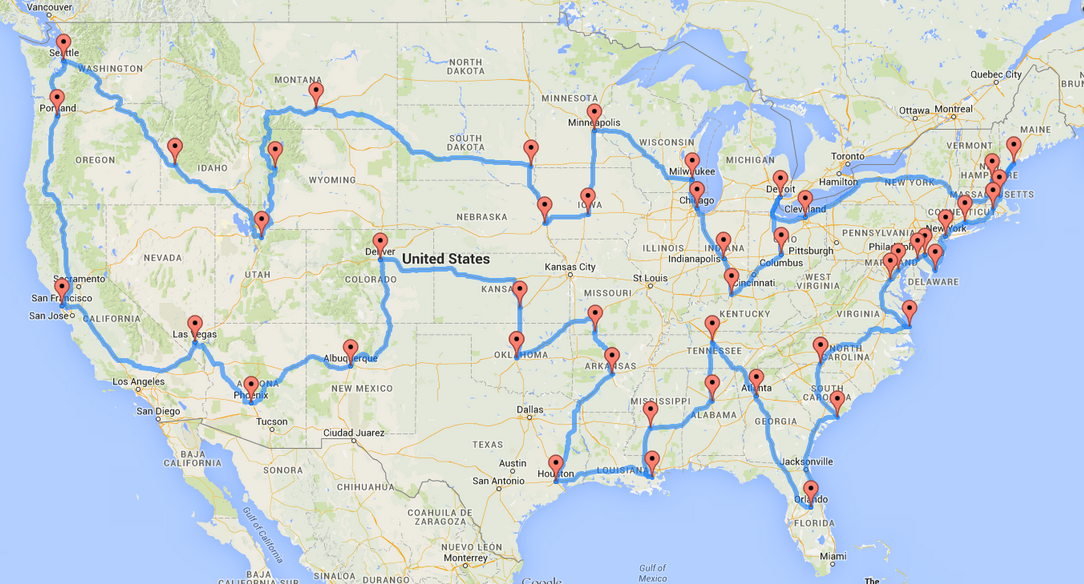
\includegraphics[width=0.9\linewidth]{images/travel_usa}
	\end{figure}
	
	\tiny Source: Randy Olson (2015)  \url{http://www.randalolson.com/2015/03/08/computing-the-optimal-road-trip-across-the-u-s/}
\end{frame}	


\begin{frame}
	
	\textbf{Isochrones} (iso = equal, chrone = time) - A buffer based on \textit{network} distances or travel times
	
	
	\begin{figure}
		\centering
		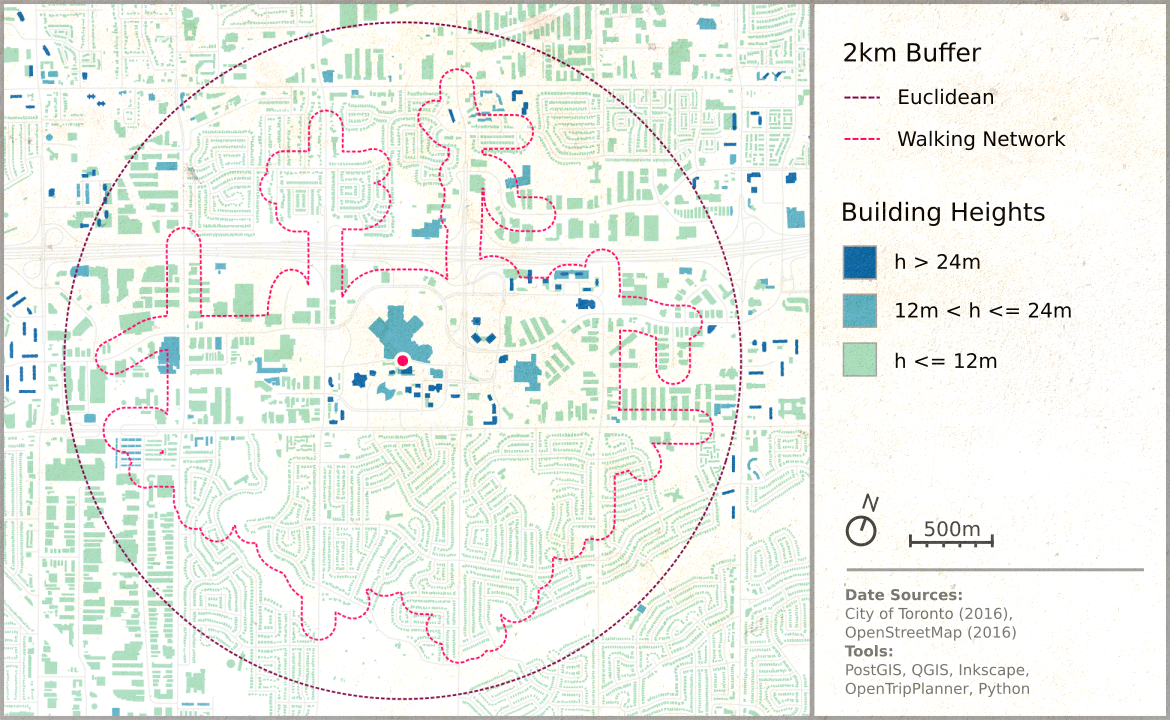
\includegraphics[width=0.8\linewidth]{images/STC_buffers}
	\end{figure}
	
	
\end{frame}



\begin{frame}
	
	
	\begin{figure}
		\centering
		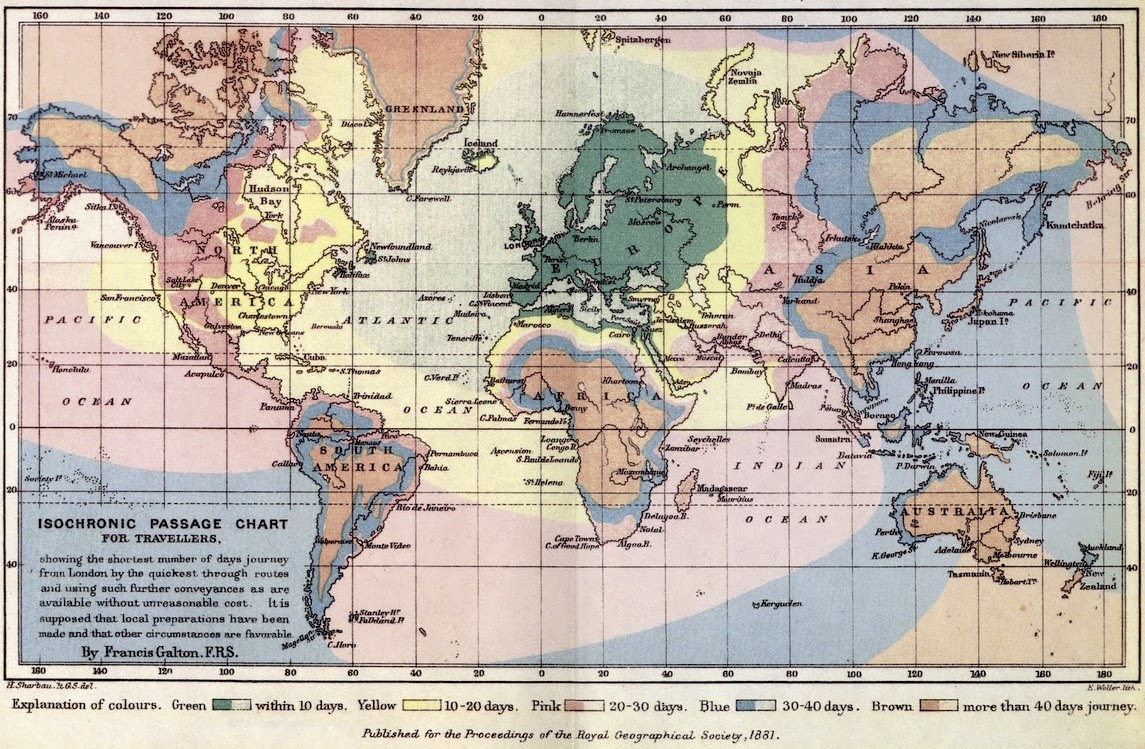
\includegraphics[width=0.8\linewidth]{images/Isochronic_Galton_1881}
	\end{figure}
	\tiny	Source:  Galton,   Francis.   1881.   "On   the   Construction   of   Isochronic   Passage-Charts." Proceedings  of  the  Royal  Geographical  Society  and Monthly Record of Geography 3: 657-658
\end{frame}




\begin{frame}
	
	\begin{figure}
		\centering
		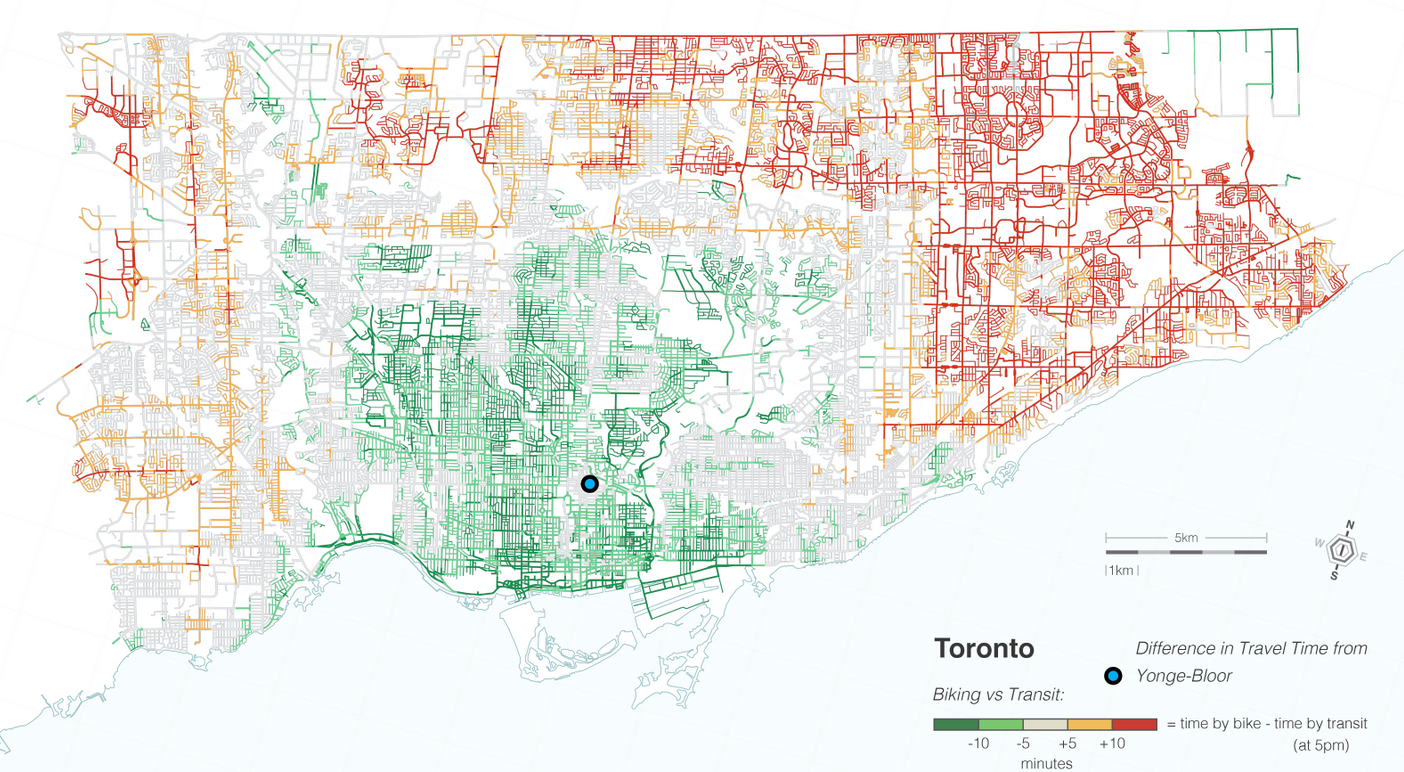
\includegraphics[width=1\linewidth]{images/bike_vs_transit}
	\end{figure}
	
	\tiny Source: Allen, J. - \textit{Using network segments in the visualization of urban isochrones} -  Cartographica - \url{http://jamaps.github.io/docs/allen_2018_isochrones.pdf}
	
\end{frame}



\begin{frame}
	
	\textbf{Origin-Destination (OD) Matrices}
	\begin{itemize}
		\item Common output of network distances/times from a set of origins to a set of destinations
		\item Also called travel time or distance matrices
		\item e.g. an isochrone can be a one-to-many OD matrix, capped at a certain threshold (e.g. 30 minutes)
	\end{itemize}
	
	\begin{figure}
		\centering
		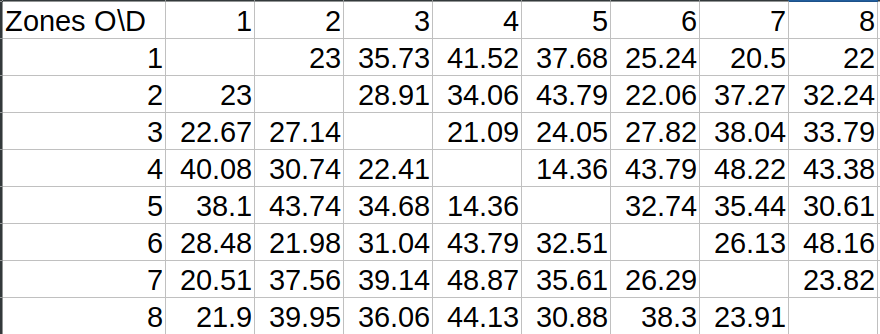
\includegraphics[width=0.66\linewidth]{images/odmatrix}
	\end{figure}
	
\end{frame}




\begin{frame}
	
	\textbf{Accessibility}

	\begin{itemize}
		\item \textit{The ease of reaching destinations}
		\item Depends on mobility (ease of travelling), but also land-use (i.e. the proximity of destinations)
		
		\item Can be measured and mapped for specific places by combining transportation network and land-use data 
		
		\item Two common measurements: 
		\begin{enumerate}
			\item minimum travel time to reach X (usually for \textit{local} analysis)
			\item how many Y can you reach in Z minutes (usually for \textit{regional} analysis)
		\end{enumerate}
	
		\item Increasingly used to evaluate transportation networks and urban livability
		
	\end{itemize}
	
\end{frame}










\begin{frame}
	
	\textbf{Measuring accessibility} - minimum travel time to reach X 
	
	(e.g. a healthy food retailer)
		
	\begin{figure}
		\centering
		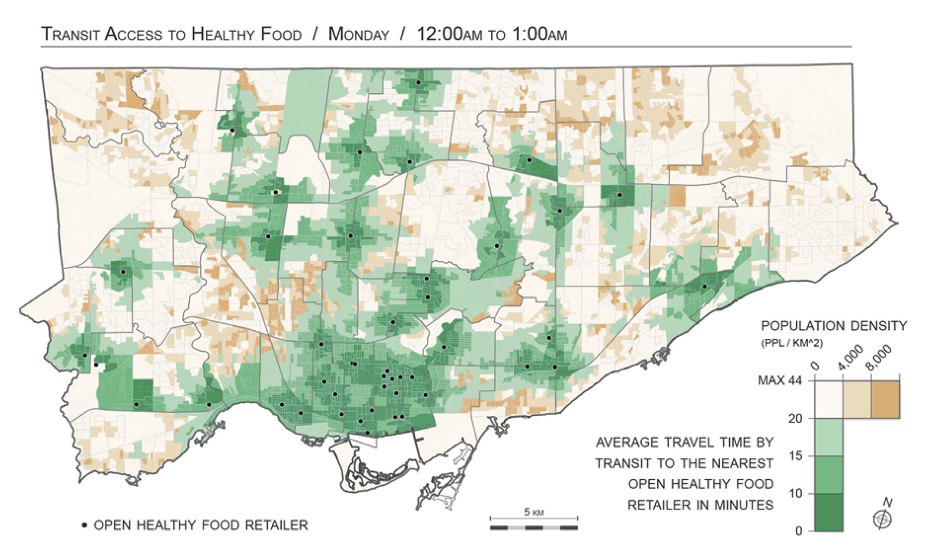
\includegraphics[width=0.86\linewidth]{images/food_midnight.png}
	\end{figure}

	\tiny Source: Widener et al (2017) How do changes in the daily food and transportation environments affect grocery store accessibility? \url{https://doi.org/10.1016/j.apgeog.2017.03.018}
	
\end{frame}



\begin{frame}
	
	\textbf{Measuring accessibility} - minimum travel time to reach X
	
	\vspace{4mm}
	
	\[A_i = \min (t_{i,j})
	\]
	
	\vspace{1mm}
		
	$A_i$ = accessibility measure for location $i$
	
	\vspace{1mm}
	
	$i$ = locations in space (e.g. grid cells, census polygons)
	
	\vspace{1mm}
	
	$j$ = location of activities (e.g. grocery store)
	
	\vspace{1mm}
	
	$t_{i,j}$ = travel cost from $i$ to $j$ (usually by computing an OD matrix)
	
\end{frame}



	

\begin{frame}
	
	\textbf{Measuring accessibility} - how many Y can you reach in Z minutes
	
	\begin{figure}
		\centering
		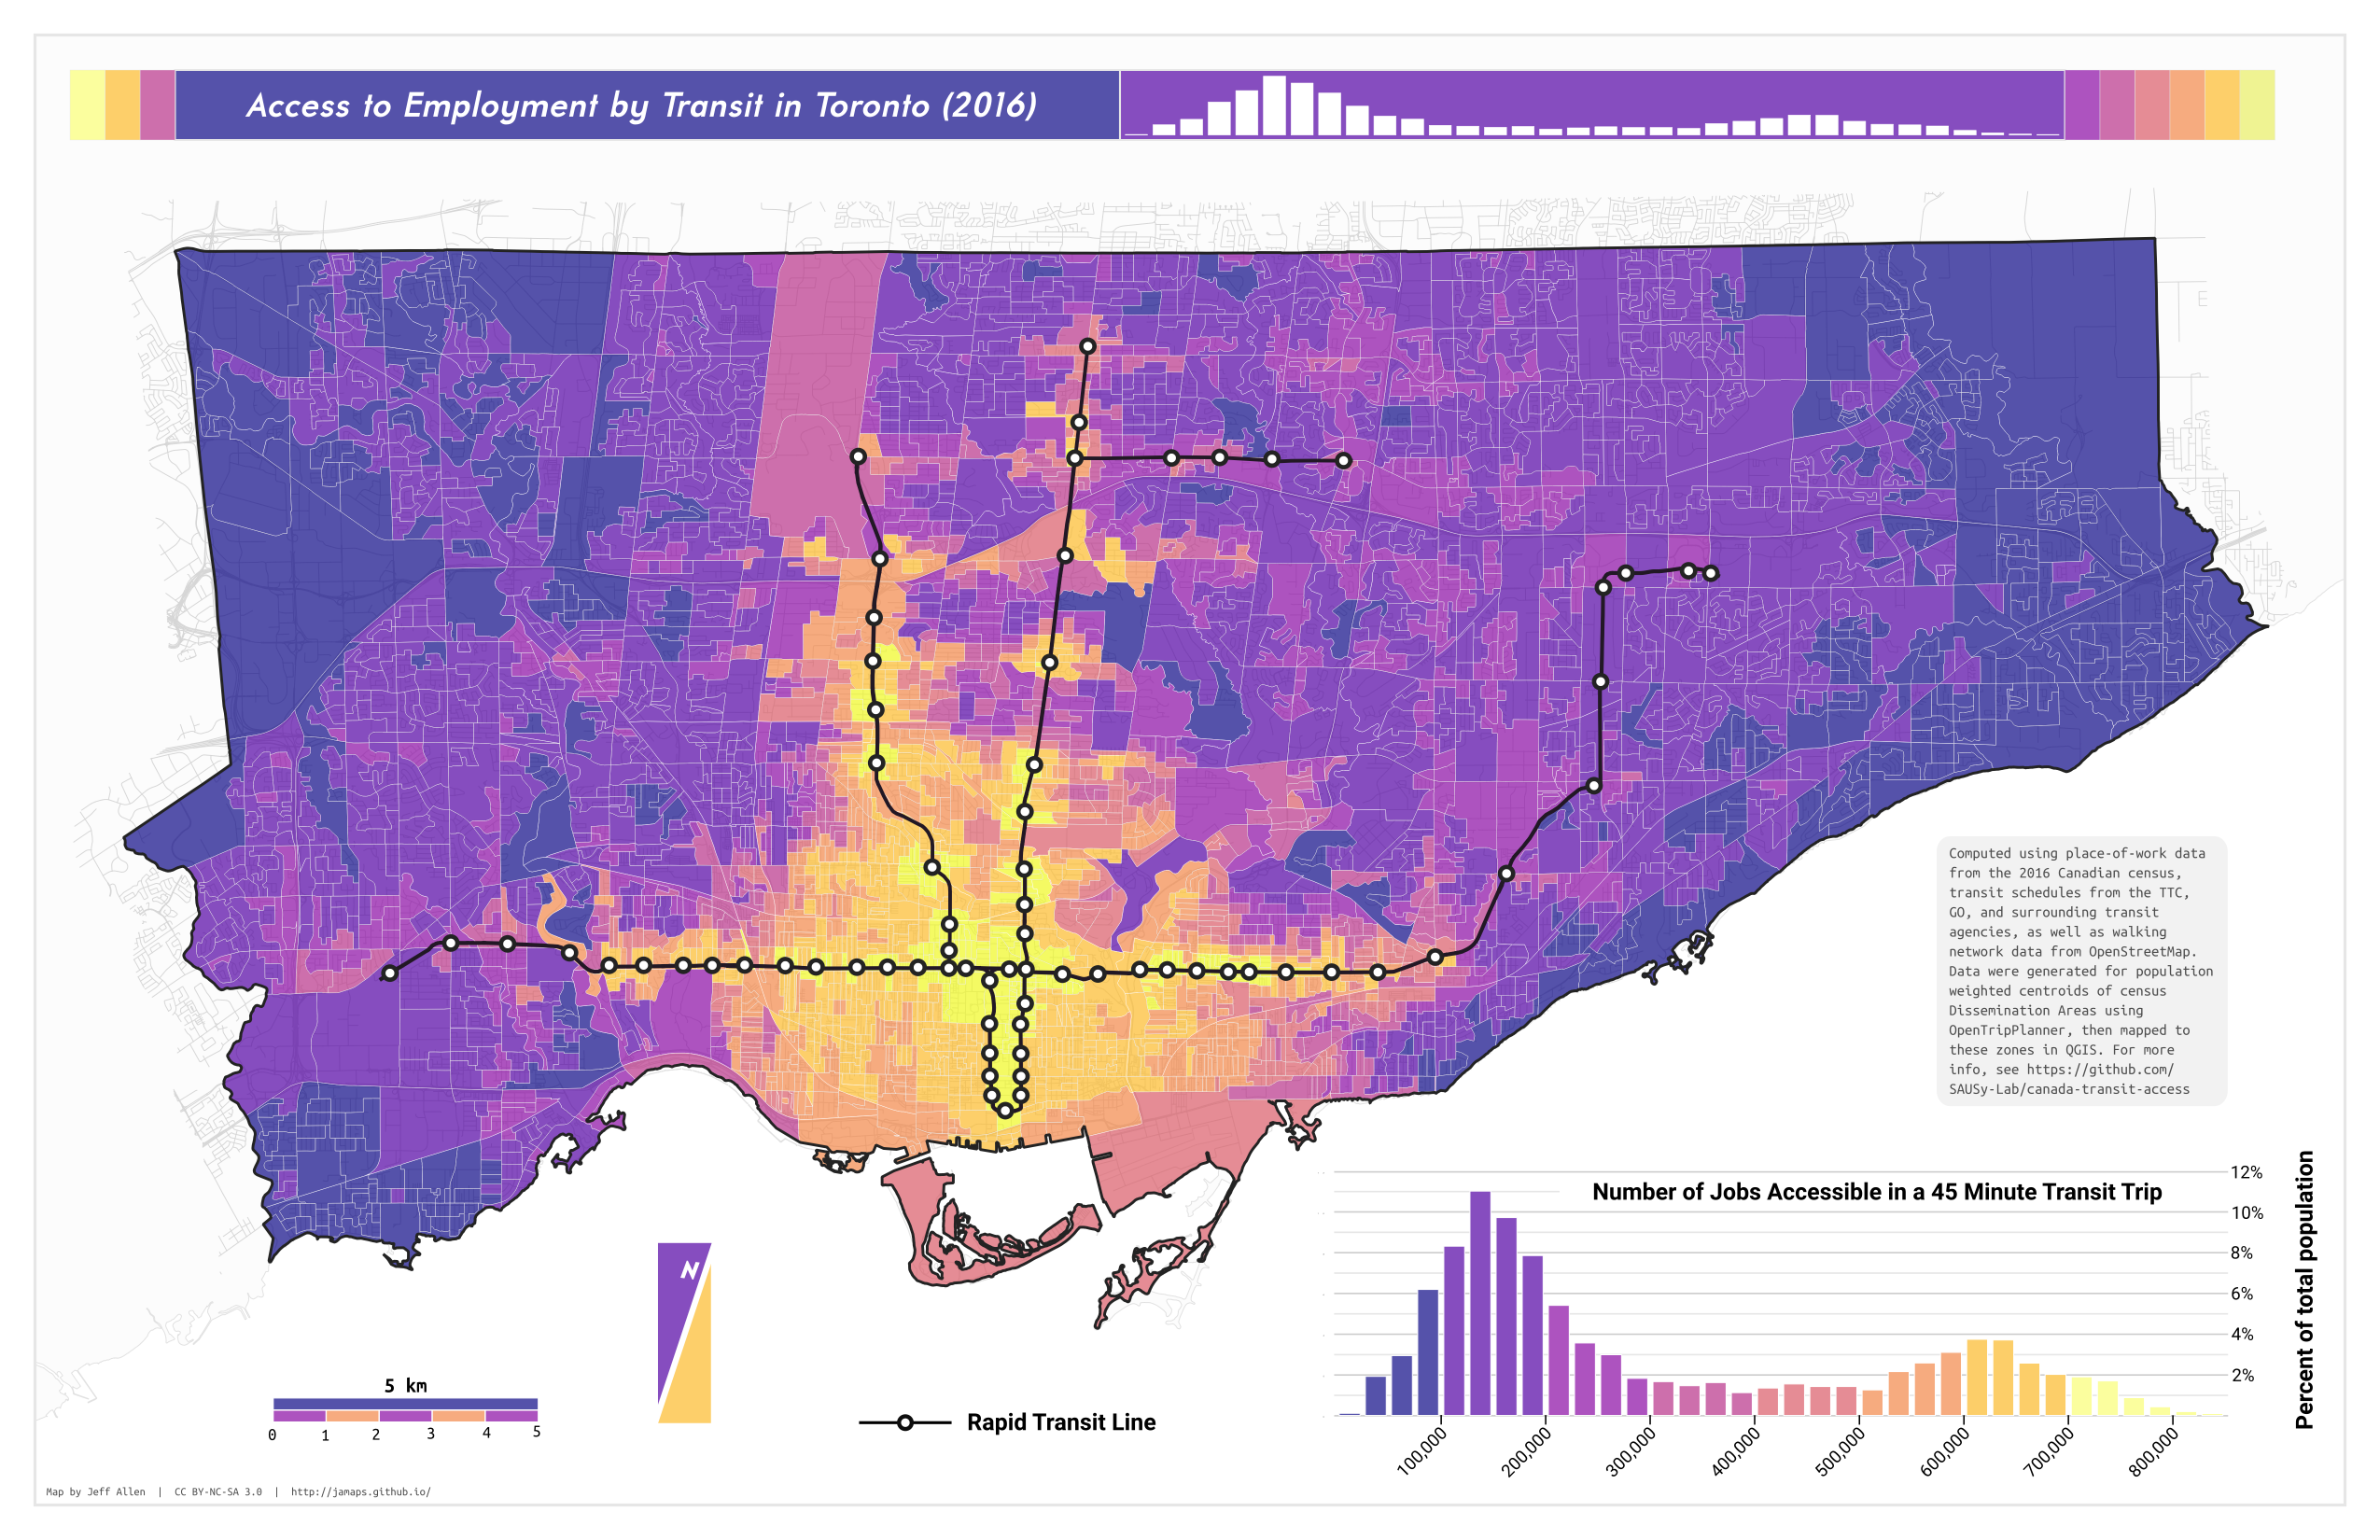
\includegraphics[width=0.86\linewidth]{images/tor_access.png}
	\end{figure}

	\tiny\url{https://en.wikipedia.org/wiki/Accessibility_(transport)}
	
\end{frame}






\begin{frame}
	
	\textbf{Measuring accessibility} - how many Y can you reach in Z minutes
	
	\vspace{1mm}
	
	\[A_i = \sum_j  f(t_{i,j}) Y_j\]
	
	
	\[
	f(t_{i,j}) = \begin{cases}
	1  & t_{i,j} \leq \theta \\
	0 & t_{i,j} > \theta
	\end{cases}\]
	
	
	\vspace{1mm}
	
	$A_i$ = accessibility measure for location $i$
	
	\vspace{1mm}
	
	$i$ = locations in space (e.g. grid cells, census polygons)
	
	\vspace{1mm}
	
	$j$ = location of activities (e.g. zones with employment counts)
	
	\vspace{1mm}
	
	$Y_j$ = number of opportunities at location $j$ (e.g. number of jobs)
	
	\vspace{1mm}
	
	$t_{i,j}$ = travel cost from $i$ to $j$ (usually by computing an OD matrix)
	
	\vspace{1mm}
	
	$f(t_{i,j})$ = \textit{impedance} function
	
	\vspace{1mm}
	
	$\theta$ = travel cost threshold (e.g. 45 minutes)
	
	
\end{frame}



\begin{frame}
	
	\textbf{Measuring accessibility} - how many Y can you reach in Z minutes
	
	\vspace{3mm}
	
	Other common \textit{impedance} functions (to try to weight nearby destinations more than those further away)
	
	\begin{figure}
		\centering
		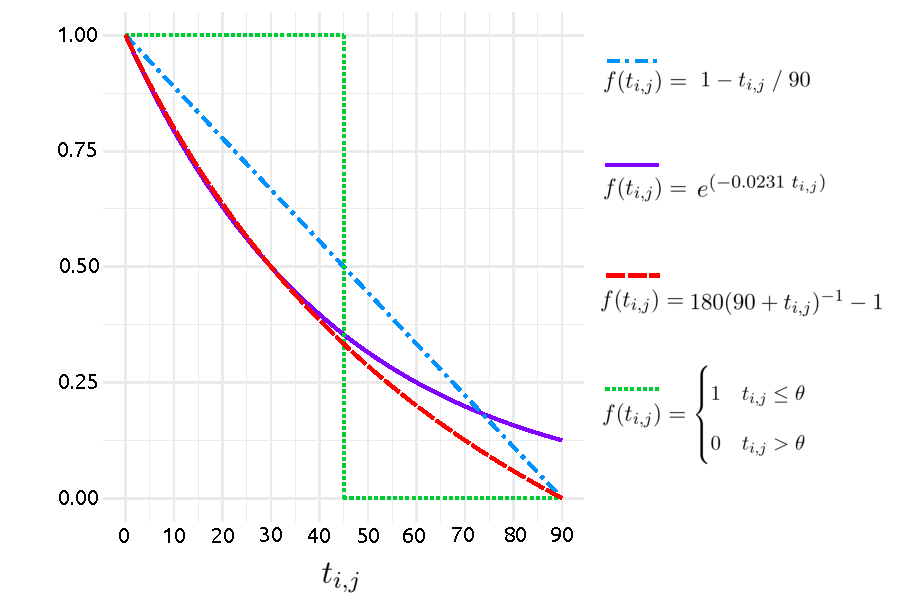
\includegraphics[width=0.76\linewidth]{images/gravity.pdf}
	\end{figure}

	
	
\end{frame}




\begin{frame}
	
	\textbf{Accessibility \& Travel Behaviour}
	
	\begin{figure}
		\centering
		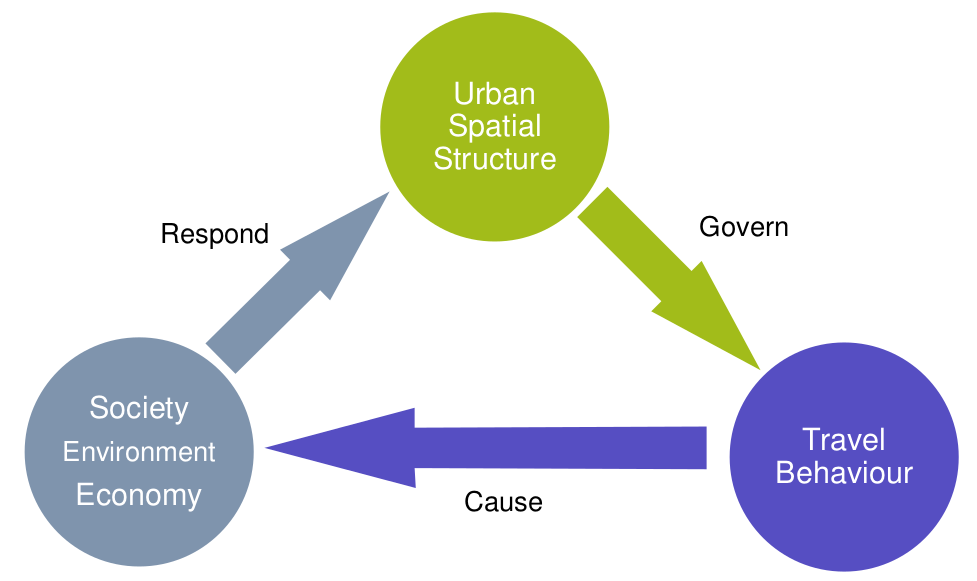
\includegraphics[width=0.56\linewidth]{images/big_links.png}
	\end{figure}
	
	
	Accessibility is correlated with ..
	\begin{itemize}
		\item Travel times
		\item Travel distances (e.g. Vehicle Kilometres Travelled)
		\item Mode share
		\item Activity participation rates
		\item Unemployment rates
	\end{itemize}
	
\end{frame}



\begin{frame}
	
	\textbf{Walkability}
	
	
	
\end{frame}



\begin{frame}
	
	\textbf{15-minute cities}
	
	
	
\end{frame}




\begin{frame}
	
	Over time historically - re commuting
	
\end{frame}



\begin{frame}
	
	Over time - Ontario Line - planning example
	
\end{frame}




\end{document}